% Chapter 8: Optimization (desirability, NSGA-II / NSGA-III, checks C and D)
\chapter{Optimization}\label{chap:8}
\label{ch:08}

The \ui{Optimization} group of the navigation tree contains four pages: \ui{Desirability}, \ui{NSGA-II / III},
\ui{Sensitivity} and \ui{Prediction \& Confirmation}. This chapter describes the first two. The \ui{Sensitivity}
page is the subject of Chapter~\ref{chap:9} and the \ui{Prediction \& Confirmation} page of Chapter~\ref{chap:10}.

Both optimization pages work on fitted models, never on the raw data. For every response you choose the model in a
\ui{Model} column: \ui{RSM} (the polynomial, GLM or split-plot model of the RSM Analysis page, Chapter~\ref{chap:5}) or
\ui{ANN} (the network trained on the ANN page, Chapter~\ref{chap:7}). The \ui{ANN} item is disabled until a network exists for
that response; its tooltip then shows the network architecture with its accuracy (``cross-validation Q2'' from
the architecture search, if one was run, and ``test R2 (single split)''), and the tooltip of \ui{RSM} shows the
predicted $R^2$ of the polynomial. The choice is stored in the project and is shared by all pages: changing the model on the
\ui{Desirability} page also changes it on the \ui{NSGA-II / III} page, in the model graphs and on the prediction
page.

The two pages answer different questions.
\begin{itemize}
  \item \textbf{Desirability} turns several responses into one score $D$ between 0 and 1 and finds the factor
        settings with the highest score. You state in advance how good each response must be and how important it
        is. The result is a short list of settings.
  \item \textbf{NSGA-II / III} keeps the objectives separate and returns the whole set of best compromises (the
        Pareto front). You see the trade-off first and choose afterwards, with help from TOPSIS and the knee point.
        The page also contains two of the diagnostic checks of REGEN: check~C (convergence and population size of
        the genetic algorithm) and check~D (comparison of the fronts obtained with the ANN and the RSM models).
\end{itemize}

% ======================================================================================================
\section{Desirability optimization}
\label{sec:ch08-desirability}

\subsection{Purpose}
The \ui{Desirability} page (page title \ui{Desirability Optimization}) finds factor settings that satisfy several
response goals at the same time, for example ``maximize yield and purity, keep cost below a limit''. Each response
is rated by an individual desirability $d_i\in[0,1]$, and the settings with the highest overall desirability $D$
are reported \citep{derringer1980,myers2016}.

\subsection{How to use}
\begin{enumerate}
  \item Fit the models first (RSM Analysis, and ANN if you want to use networks). A response without a model is
        skipped with the message \ui{Skipped responses without a model: \dots}.
  \item Open \ui{Desirability} in the navigation tree. The upper group \ui{Optimization Criteria} lists one row
        per factor, one row per response and, when factor standard deviations have been entered (Chapter~\ref{chap:4},
        \ui{Factor \& Response Info\dots}), one \ui{POE} row per response.
  \item In the factor rows, narrow the \ui{Lower Limit} and \ui{Upper Limit} if the search should stay inside a
        smaller region. The limits are in actual units.
  \item In each response row choose a \ui{Goal}, edit the limits (and the \ui{Target} for the goal
        \ui{Target}), and set \ui{Shape}, \ui{Importance} and \ui{Model}.
  \item Click \ui{Run Optimization}. The solutions appear in the group \ui{Solutions (Sorted by Desirability)},
        and the bar chart on the right shows the individual and combined desirability of the selected row.
  \item Select a row and click \ui{Send Selected Solution to Prediction} to obtain confidence and prediction
        intervals and to plan confirmation runs (Chapter~\ref{chap:10}).
\end{enumerate}
\ui{Reset Limits to Data} refills all limits and targets with their defaults. The criteria are saved in the project,
and the \ui{NSGA-II / III} page takes its factor limits, goals and targets from them.

\subsection{Options}
Table~\ref{tab:ch08-desir-options} lists the columns of the criteria table.

\begin{table}[htbp]
\centering
\small
\caption{Columns of the \ui{Optimization Criteria} table on the \ui{Desirability} page.}
\label{tab:ch08-desir-options}
\begin{tabularx}{\linewidth}{@{}>{\raggedright\arraybackslash}p{3.0cm} >{\raggedright\arraybackslash}p{3.4cm} >{\raggedright\arraybackslash}p{2.3cm} >{\raggedright\arraybackslash}X@{}}
\toprule
Column & Values & Default & Meaning \\
\midrule
\ui{Goal} (factor) & \ui{In range} (numeric), \ui{All levels} (categoric) & fixed & Numeric factors are searched
between their limits; every level combination of the categoric factors is optimized separately. \\
\ui{Lower Limit}, \ui{Upper Limit} (factor) & numbers in actual units & factor low and high & Search region. \\
\ui{Goal} (response) & \ui{None}, \ui{Maximize}, \ui{Minimize}, \ui{Target}, \ui{In range} & \ui{None} & \ui{None}
leaves the response out of $D$. \\
\ui{Lower Limit}, \ui{Upper Limit} (response) & numbers & data minimum and maximum & $L$ and $U$ in
Eqs.~\eqref{eq:ch08-dmax}--\eqref{eq:ch08-drange}. For a binomial response the proportion (count / trials) is
used. \\
\ui{Target} & number between the limits & midpoint of the data range & $T$ for the goal \ui{Target}; ignored for the
other goals. \\
\ui{Shape} & 0.10--10.00, step 0.1 & 1.00 & Shape exponent $s$ of the desirability ramp (1 = linear). \\
\ui{Importance} & \ui{+} \dots\ \ui{+++++} (1--5) & \ui{+++} (3) & Weight $r_i$ in the geometric mean
\eqref{eq:ch08-D}. \\
\ui{Model} & \ui{RSM}, \ui{ANN} & \ui{RSM} & Model used to predict the response (project-wide choice). POE rows show
\ui{follows response}. \\
\bottomrule
\end{tabularx}
\end{table}

For a \ui{POE} row the default limits are 0 and the largest POE value over the design points; the usual goal is
\ui{Minimize}, which favors settings where the response is insensitive to small variations of the factors.

\subsection{Output and how to read it}
The solutions table has the columns \ui{No}, the factors (actual units), all responses (predicted with the model
selected for each response) and \ui{Desirability}. At most 20 solutions are listed; row~1, the best, is shaded
green. Solutions that lie within 0.03 coded units of a better one are removed, so the rows are genuinely different
settings. When all starts converge to the same point you get a single row; several rows with nearly the same $D$
indicate a flat optimum, where you may choose the most convenient setting.

The bar chart (title \ui{Desirability of solution $k$}) shows each $d_i$ in blue and the combined $D$ in green.
A response with $d_i$ close to 0 is the bottleneck; relaxing its limits or lowering the importance of the other
responses changes the compromise most.

Messages (title \ui{Optimization}):
\begin{itemize}
  \item \ui{Some limits are not numbers.}, \ui{Invalid limits for factor \dots}, \ui{Limits for response \dots:
        lower must be < upper.}, \ui{The target for \dots\ must be between the limits.}: correct the table.
  \item \ui{Choose a goal (Maximize/Minimize/Target/In range) for at least one response whose model is
        available.}: no response is active.
  \item \ui{The component limits do not allow the mixture to sum to the total.}: for mixtures, the lower limits sum
        to more than the total (or the upper limits to less).
  \item \ui{No point satisfies all limits and constraints.}: none of the random points satisfies the linear
        constraints of the design together with the factor limits; widen the limits.
\end{itemize}

\subsection{Theory as implemented}
Let $y_i(\mathbf x)$ be the prediction of response $i$ at the factor setting $\mathbf x$ (coded units), $L_i$ and
$U_i$ its limits, $T_i$ its target and $s_i$ its shape exponent. REGEN uses the desirability functions of
\citet{derringer1980}:
\begin{align}
\text{Maximize:}\quad & d_i=\left[\operatorname{clip}\!\left(\frac{y_i-L_i}{U_i-L_i},0,1\right)\right]^{s_i},
\label{eq:ch08-dmax}\\
\text{Minimize:}\quad & d_i=\left[\operatorname{clip}\!\left(\frac{U_i-y_i}{U_i-L_i},0,1\right)\right]^{s_i},
\label{eq:ch08-dmin}\\
\text{Target:}\quad & d_i=\begin{cases}
\left(\dfrac{y_i-L_i}{T_i-L_i}\right)^{s_i}, & L_i\le y_i\le T_i,\\[2ex]
\left(\dfrac{U_i-y_i}{U_i-T_i}\right)^{s_i}, & T_i< y_i\le U_i,\\[1ex]
0, & \text{otherwise,}\end{cases}
\label{eq:ch08-dtarget}\\
\text{In range:}\quad & d_i=\begin{cases}1, & L_i\le y_i\le U_i,\\ 0, & \text{otherwise,}\end{cases}
\label{eq:ch08-drange}
\end{align}
where $\operatorname{clip}(u,0,1)$ limits $u$ to $[0,1]$. With $s_i=1$ the ramp is linear; with $s_i>1$ the
response must come close to the goal before $d_i$ rises; with $s_i<1$ the desirability rises quickly away from the
limit. The original paper allows different exponents on the two sides of a target; REGEN uses the same exponent
on both sides. A prediction that is not a number gives $d_i=0$.

Note the consequence of the clipping in \eqref{eq:ch08-dmax}: once $y_i\ge U_i$ the response is fully desirable,
and the search no longer tries to increase it. With the default limits (data minimum and maximum), maximizing a
response means ``reach at least the best observed value''. If you want the search to go further, raise $U_i$, but
remember that predictions beyond the observed range are extrapolations.

The overall desirability is the importance-weighted geometric mean
\begin{equation}
D(\mathbf x)=\left(\prod_{i} d_i^{\,r_i}\right)^{1/\sum_i r_i}
=\exp\!\left(\frac{\sum_i r_i\ln d_i}{\sum_i r_i}\right),\qquad D=0\ \text{if any}\ d_i=0,
\label{eq:ch08-D}
\end{equation}
with $r_i\in\{1,\dots,5\}$ the importance. Responses with goal \ui{None} are left out. Because $D$ is a geometric
mean, a single unacceptable response ($d_i=0$) makes the whole setting unacceptable.

The search proceeds as follows (\texttt{doe/optimize.py} and \texttt{Project.optimize}):
\begin{enumerate}
  \item The factor limits are converted to coded units (for mixtures intersected with the component bounds).
        Each combination of categoric factor levels is optimized separately with
        $n_\text{starts}=\max(8,\lfloor 30/n_\text{comb}\rfloor)$ starts ($n_\text{comb}$ = number of level
        combinations; 30 starts without categoric factors).
  \item 4000 random points are drawn uniformly in the limits (12\,000 when the design has linear constraints, of
        which the feasible ones are kept, at most 4000). For mixtures the points are drawn uniformly on the simplex
        above the lower bounds and filtered by the upper bounds. The random generator has a fixed seed (0), so the
        same criteria always give the same solutions.
  \item The $n_\text{starts}$ points with the highest $D$ become starting points of a local search: Nelder--Mead
        with bounds (tolerances $10^{-5}$ in $\mathbf x$ and $10^{-8}$ in $D$, at most 2000 iterations) for an
        unconstrained process design, and SLSQP (at most 300 iterations) with the mixture equality
        $\sum x_\text{comp}=1$ and the linear constraints $G\mathbf x\le\mathbf h$ otherwise. An infeasible point
        scores $D=0$, and SLSQP results that are worse than their start are replaced by the start.
  \item All end points are sorted by $D$; points within a Euclidean distance of 0.03 (coded units) of a better
        point are removed; the 20 best are shown.
\end{enumerate}

\textbf{POE criterion.} When standard deviations $\sigma_j$ of the factors have been entered, the propagation of
error of response $i$ is
\begin{equation}
\text{POE}_i(\mathbf x)=\sqrt{\sum_j\left(\frac{\partial y_i}{\partial x_j}\right)^2\sigma_{x,j}^2
+\left(\frac{\partial y}{\partial\eta}\right)^2\sigma^2_\text{resid}},
\label{eq:ch08-poe}
\end{equation}
where $\sigma_{x,j}$ is the factor standard deviation in coded units, the derivatives are central differences with
step $10^{-4}$, $\eta$ is the (possibly transformed) model scale and $\sigma^2_\text{resid}$ is the residual mean
square of the RSM model (for an ANN, its mean squared error on all data). The POE row uses the model of its response.
POE is described in more detail in Chapter~\ref{chap:6}.

\textbf{Limitations.} The optimizer is a multi-start local search. It is reliable for the smooth models of RSM,
but for an ANN with many local optima increase the confidence by comparing with the NSGA front
(Section~\ref{sec:ch08-nsga}). The result is an optimum of the \emph{model}; it must be confirmed by experiments.

\subsection{Example: BBD extraction}
\label{sec:ch08-desir-example}
Case study \ui{Extraction Optimization (Box-Behnken)} (Temperature 60--80~°C, Time 30--90~min,
Concentration 1--3~\%, responses Yield and Purity, both fitted with the quadratic RSM model). Both responses are set
to \ui{Maximize} with lower limits 75 (Yield) and 89 (Purity); the upper limits stay at the data maxima 78.29 and
93.6, shape 1.00, importance \ui{+++}, model \ui{RSM} (Figure~\ref{fig:ch08-desirability}).

\begin{figure}[htbp]
\centering
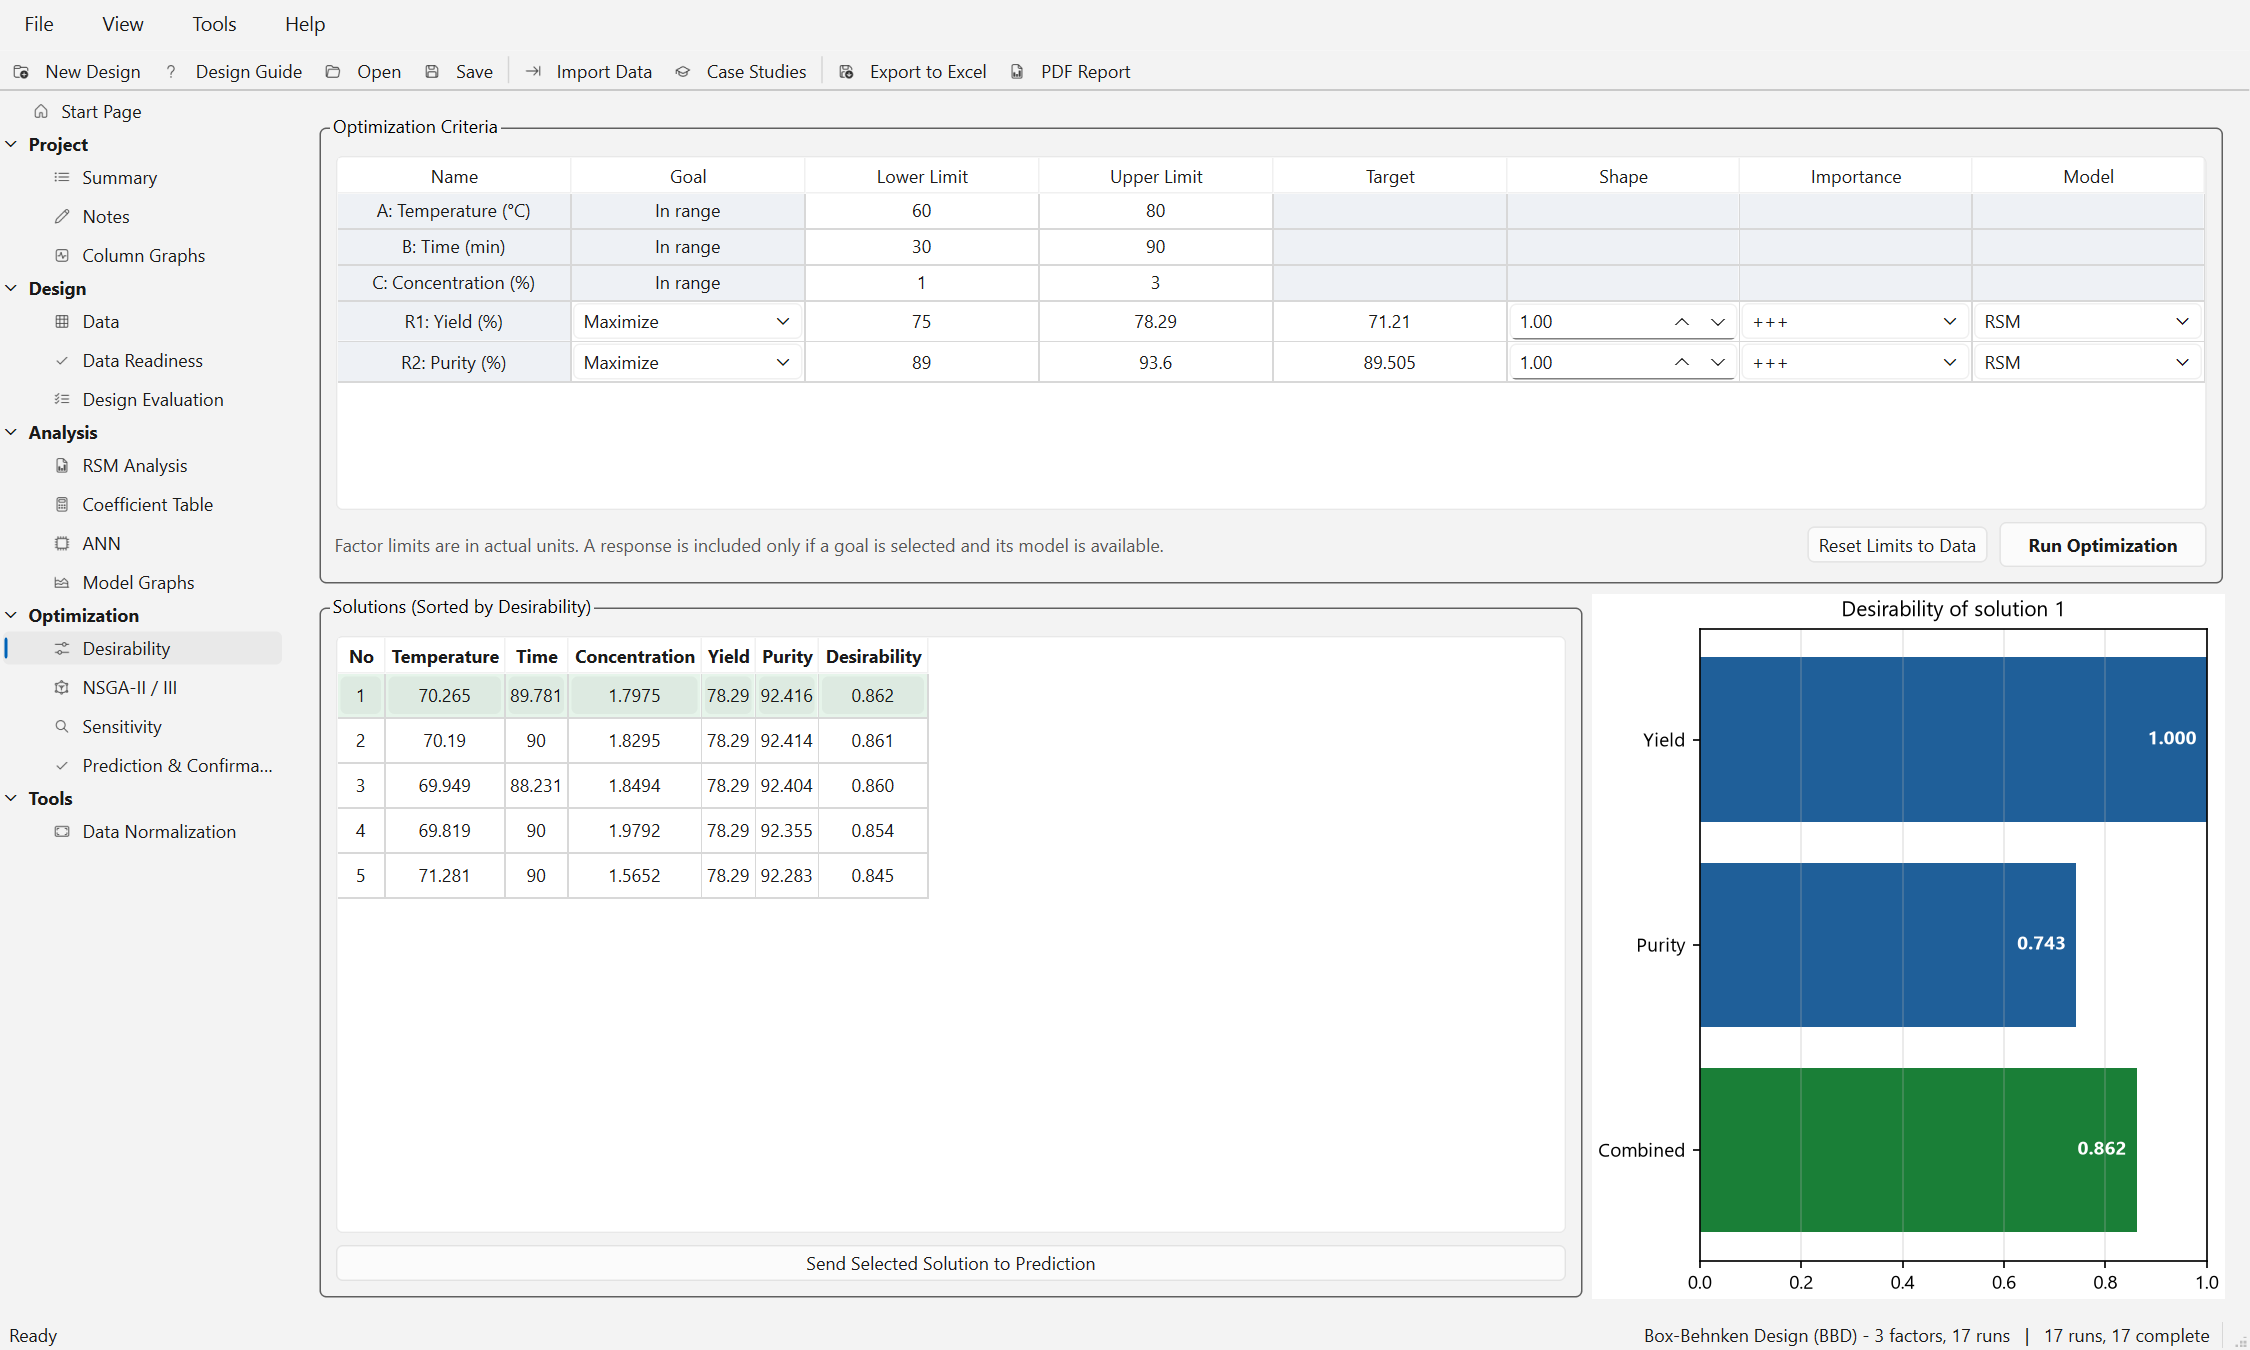
\includegraphics[width=\linewidth]{desirability.png}
\caption{\ui{Desirability} page for the BBD extraction case: Yield and Purity maximized (limits 75--78.29 and
89--93.6). Five distinct solutions; the best, at 70.265~°C, 89.781~min and 1.7975~\%, has $D=0.862$.}
\label{fig:ch08-desirability}
\end{figure}

\ui{Run Optimization} returns five distinct solutions with $D$ between 0.845 and 0.862. The best one is
Temperature 70.265~°C, Time 89.781~min, Concentration 1.7975~\%, with predicted Yield 78.29 and Purity 92.416. The
bar chart shows $d_\text{Yield}=1.000$, $d_\text{Purity}=(92.416-89)/(93.6-89)=0.743$ and
$D=\sqrt{1.000\times0.743}=0.862$ (equal importances, so $D$ is the plain geometric mean).

Yield sits exactly at its upper limit 78.29 in all five rows: once Yield reaches the data maximum its desirability
is 1, so the optimizer spends the remaining freedom on Purity. The five rows differ mainly in Concentration
(1.57--1.98~\%), which shows that the optimum is flat in that direction. The NSGA front below shows that the model
predicts Yield up to about 80.4 for lower Purity.

\textbf{Data export.} Right-click the solutions table for \ui{Copy selected cells}, \ui{Copy entire table (for
Excel)} and \ui{Export table\dots}; right-click the bar chart for \ui{Copy plot data} and \ui{Export plot
data\dots}. The solutions are saved with the project.

% ======================================================================================================
\section{Multi-objective optimization: NSGA-II and NSGA-III}
\label{sec:ch08-nsga}

\subsection{Purpose}
The \ui{NSGA-II / III} page (page title \ui{Multi-objective Optimization (NSGA-II / NSGA-III)}) finds the Pareto
front: the set of factor settings for which no objective can be improved without making another one worse. It is
the right tool when the responses conflict and you want to see the trade-off before deciding
\citep{chapman2014}. A compromise is then picked by TOPSIS \citep{hwang1981} or at the knee of the front.

\subsection{How to use}
\begin{enumerate}
  \item Set the factor limits on the \ui{Desirability} page if the search region should be smaller than the design
        range (the NSGA page uses those limits; the note on the page says ``Factor limits are taken from the
        Desirability page.'').
  \item In the group \ui{Objectives \& Constraints (Select at Least 2 Objectives)} choose for each response the
        \ui{Model} and the \ui{Goal} (\ui{Ignore}, \ui{Maximize}, \ui{Minimize}, \ui{Target}). Goals and targets are
        pre-filled from the \ui{Desirability} page when the goal there is \ui{Maximize}, \ui{Minimize} or
        \ui{Target}.
  \item Optionally enter \ui{Lower limit (constraint)} and \ui{Upper limit (constraint)} for any response (empty
        means no limit). A row with goal \ui{Ignore} and a limit becomes a pure constraint.
  \item Optionally change the \ui{TOPSIS weight} of each objective (default 1).
  \item Check the algorithm parameters (Table~\ref{tab:ch08-nsga-options}) and click \ui{Run Optimization}. The
        progress text reads \ui{generation $g$ of max $G$}; \ui{Stop} ends the run early.
  \item Read the front in the \ui{Graph} tab and the convergence check in the \ui{Convergence \& Adequacy} tab.
        Click \ui{Check Population Size} to complete check~C.
  \item If ANN models exist, click \ui{Compare ANN vs RSM} (check~D, Section~\ref{sec:ch08-checkD}).
  \item Select a row of the solutions table and click \ui{Send Selected Solution to Prediction} (without a selection
        the TOPSIS solution is sent).
\end{enumerate}

\subsection{Options}
\begin{table}[htbp]
\centering
\small
\caption{Settings of the \ui{NSGA-II / III} page.}
\label{tab:ch08-nsga-options}
\begin{tabularx}{\linewidth}{@{}>{\raggedright\arraybackslash}p{3.4cm} >{\raggedright\arraybackslash}p{3.6cm} >{\raggedright\arraybackslash}p{2.2cm} >{\raggedright\arraybackslash}X@{}}
\toprule
Setting & Values & Default & Meaning \\
\midrule
\ui{Model} & \ui{RSM}, \ui{ANN} & \ui{RSM} & Model of each response; POE rows show \ui{RSM + POE} or
\ui{ANN + POE}. \\
\ui{Goal} & \ui{Ignore}, \ui{Maximize}, \ui{Minimize}, \ui{Target} & from Desirability & At least two objectives
are required. \\
\ui{Target} & number & from Desirability & Required for the goal \ui{Target}. \\
\ui{Lower/Upper limit (constraint)} & number or empty & empty & Response constraints, Eq.~\eqref{eq:ch08-cv}. \\
\ui{TOPSIS weight} & positive number & 1 & Weight $w_k$ in TOPSIS, Eq.~\eqref{eq:ch08-topsis}. \\
\ui{Population:} & 20--2000 & 100 & Population size $N$ (rounded up to an even number). \\
\ui{Max generations:} & 10--10\,000 & 300 & Upper limit of the number of generations. \\
\ui{P crossover:} & 0.10--1.00 & 0.90 & Probability $p_c$ that a parent pair is crossed. \\
\ui{$\eta$ crossover:} & 1--100 & 15 & Distribution index $\eta_c$ of SBX. \\
\ui{$\eta$ mutation:} & 1--100 & 20 & Distribution index $\eta_m$ of polynomial mutation. \\
\ui{Seed:} & 0--999\,999 & 1 & Random seed; the same seed gives the same front. \\
\ui{Algorithm:} & \ui{Automatic (NSGA-III for 3 or more objectives)}, \ui{NSGA-II}, \ui{NSGA-III (reference
points)} & Automatic & See Section~\ref{sec:ch08-auto}. \\
\ui{Stop automatically on convergence} & on/off & on & Window stopping rule of check~C. \\
\ui{tolerance:} & 0.001--5.000~\% & 0.100~\% & Tolerance $\tau_0$ of the hypervolume gain. \\
\ui{within} & 5--500 generations & 20 & Window length $w$. \\
\bottomrule
\end{tabularx}
\end{table}
The mutation probability per variable is $p_m=1/n$ ($n$ = number of factors); it is not shown on the page.

\subsection{Problem formulation}
The decision variables are the factors in coded units. Their bounds are the coded design range intersected with
the factor limits of the \ui{Desirability} page (for mixtures, clipped to the component bounds). Categoric factors
are integer variables $0,\dots,L-1$. All objectives are minimized internally:
\begin{equation}
F_k(\mathbf x)=\begin{cases}-y_k(\mathbf x) & \text{Maximize},\\ y_k(\mathbf x) & \text{Minimize},\\
|y_k(\mathbf x)-T_k| & \text{Target.}\end{cases}
\label{eq:ch08-F}
\end{equation}
The graphs and tables always show the response values $y_k$, not $F_k$. Response limits, linear design constraints
$G\mathbf x\le\mathbf h$ and the mixture sum enter a total constraint violation
\begin{equation}
\begin{split}
CV(\mathbf x)={}&\sum_o\frac{\max(0,L_o-y_o)+\max(0,y_o-U_o)}{s_o}+\sum_r\max\bigl(0,(G\mathbf x-\mathbf h)_r\bigr)\\
&+\Bigl|\sum_{c}x_c-1\Bigr|\,\mathbb 1\!\left[\Bigl|\sum_c x_c-1\Bigr|>10^{-6}\right],
\end{split}
\label{eq:ch08-cv}
\end{equation}
where the first sum runs over the responses with a limit, $s_o=|U_o-L_o|$ when both limits are given and
otherwise the standard deviation of $y_o$ in the current population (at least $10^{-9}$), and the last term
applies to mixture components $c$. A setting is feasible when $CV=0$. For mixtures every new individual is first
repaired: the components are clipped to their bounds and the deficit $1-\sum x_c$ is shared in proportion to the
remaining room, up to 30 times.

\subsection{NSGA-II}
NSGA-II \citep{deb2002} evolves a population of $N$ settings. REGEN implements it as follows.
\begin{description}[style=nextline]
  \item[Initialization] $N$ settings uniform in the bounds (integers rounded, mixtures repaired).
  \item[Constraint domination] Setting $a$ dominates $b$ if both are feasible and $F_k(a)\le F_k(b)$ for all $k$
        with at least one strict inequality; or $a$ is feasible and $b$ is not; or both are infeasible and
        $CV(a)<CV(b)$ \citep{deb2002}.
  \item[Non-dominated sorting] The population is peeled into fronts: rank~0 contains the settings dominated by
        none, rank~1 those dominated only by rank~0, and so on.
  \item[Crowding distance] Within each front and for each objective $k$, the members are sorted by $F_k$; the two
        boundary members get $\infty$ and each inner member $i$ adds
        \begin{equation}
        c_i\mathrel{+}=\frac{F_{k}^{(i+1)}-F_{k}^{(i-1)}}{F_{k}^{\max}-F_{k}^{\min}}.
        \label{eq:ch08-crowding}
        \end{equation}
        Fronts with at most two members get $\infty$. A large $c_i$ means an isolated point that keeps the front
        spread out.
  \item[Parent selection] Binary tournament: of two random members the lower rank wins, and at equal rank the
        larger crowding distance.
  \item[Crossover (SBX)] Each parent pair is crossed with probability $p_c$; each variable of the pair with
        probability 0.5 (not when the parents are equal or the bound is degenerate). With parents $x_1<x_2$, bounds
        $[l,u]$ and a uniform random number $\upsilon$, the bounded simulated binary crossover used in NSGA-II is
        \begin{align}
        \beta&=1+\frac{2\min(x_1-l,\;u-x_2)}{x_2-x_1},\qquad \alpha=2-\beta^{-(\eta_c+1)},\nonumber\\
        \beta_q&=\begin{cases}(\upsilon\alpha)^{1/(\eta_c+1)}, & \upsilon\le 1/\alpha,\\
        \bigl(1/(2-\upsilon\alpha)\bigr)^{1/(\eta_c+1)}, & \text{otherwise,}\end{cases}\label{eq:ch08-sbx}\\
        c_{1,2}&=\tfrac12\bigl[(x_1+x_2)\mp\beta_q(x_2-x_1)\bigr],\nonumber
        \end{align}
        clipped to the bounds; the two children are swapped with probability 0.5. A large $\eta_c$ keeps the children
        close to the parents. Integer variables are crossed the same way and rounded.
  \item[Mutation (polynomial)] Each variable mutates with probability $p_m=1/n$. With
        $\delta_1=(x-l)/(u-l)$, $\delta_2=(u-x)/(u-l)$ and a uniform $\upsilon$,
        \begin{equation}
        \delta_q=\begin{cases}
        \bigl[2\upsilon+(1-2\upsilon)(1-\delta_1)^{\eta_m+1}\bigr]^{1/(\eta_m+1)}-1, & \upsilon<0.5,\\
        1-\bigl[2(1-\upsilon)+2(\upsilon-0.5)(1-\delta_2)^{\eta_m+1}\bigr]^{1/(\eta_m+1)}, & \text{otherwise,}
        \end{cases}
        \label{eq:ch08-pm}
        \end{equation}
        and $x\leftarrow\operatorname{clip}(x+\delta_q(u-l),l,u)$. Integer variables are reset to a random level.
  \item[Survival] Parents and children ($2N$) are sorted by rank and, within a rank, by decreasing crowding
        distance; the first $N$ survive (elitism).
  \item[Result] The feasible rank-0 members of the last generation, without duplicates (rounded to 8 decimals),
        sorted by the first objective.
\end{description}

\subsection{NSGA-III}
With three or more objectives almost every member of the population is non-dominated, and the crowding distance can
no longer separate them. NSGA-III \citep{deb2014} keeps the front evenly spread with a set of reference directions.
REGEN implements it as follows.
\begin{description}[style=nextline]
  \item[Reference directions] Das--Dennis points \citep{das1998}: all vectors $\boldsymbol\lambda$ with components
        $j/H$ ($j=0,\dots,H$) that sum to 1. For $m$ objectives there are
        \begin{equation}
        R=\binom{H+m-1}{m-1}
        \label{eq:ch08-refs}
        \end{equation}
        points; REGEN chooses the largest $H$ with $R\le N$. Example: $m=3$, $N=100$ gives $H=12$ and $R=91$.
  \item[Selection] Fronts are added whole while they fit into $N$. If the last front that does not fit is infeasible,
        its members with the smallest $CV$ are taken. Otherwise the members are chosen by niching (below).
  \item[Normalization] The ideal point $\mathbf z^*$ (minimum of each objective over the candidates) is subtracted,
        $F'=F-\mathbf z^*$. For each axis $k$ the extreme point minimizes the achievement scalarizing function
        $\max_j F'_j/w_j$ with $w_k=1$ and $w_j=10^{-6}$ otherwise. The intercepts $a_k$ of the hyperplane through
        the $m$ extreme points ($E\mathbf b=\mathbf 1$, $a_k=1/b_k$) normalize the objectives, $F^z=F'/\mathbf a$.
        When the system is singular or gives intercepts $\le10^{-10}$, the maximum of $F'$ per objective is used.
  \item[Association] Each candidate is assigned to the reference direction $\mathbf u_j$ (unit vector) with the
        smallest perpendicular distance $d_\perp^2=\|F^z\|^2-(F^z\cdot\mathbf u_j)^2$.
  \item[Niching] The niche count $\rho_j$ is the number of already selected members per direction. Repeatedly, a
        direction with the smallest $\rho_j$ among those with candidates is chosen (ties at random); if $\rho_j=0$
        its closest candidate is taken, otherwise a random one; then $\rho_j$ increases by one.
  \item[Parent selection] In NSGA-III the crowding distance in the tournament is replaced by a random number, so
        parents of the same rank are paired at random.
\end{description}
SBX, polynomial mutation and constraint domination are the same as in NSGA-II.

\subsection{Automatic choice of the algorithm}
\label{sec:ch08-auto}
With \ui{Automatic (NSGA-III for 3 or more objectives)} REGEN uses NSGA-II for two objectives and NSGA-III for three
or more (counting the rows with a goal other than \ui{Ignore}). Constraint-only rows do not count. You can force
either algorithm; the tooltip summarizes the reason: \ui{NSGA-II uses crowding distance; good for 2 objectives.
NSGA-III uses reference points so solutions stay evenly spread for 3 or more objectives}.

\subsection{Response limits as constraints}
A limit turns the corresponding part of the response range into an infeasible region; infeasible settings always
lose against feasible ones. Example (BBD case): with Yield and Purity maximized and a \ui{Lower limit (constraint)}
of 92 for Purity, NSGA-II (seed 1) stops at generation 76 with 99 solutions. All of them have Purity
$\ge92.006$; Yield ranges from 63.6 to 78.9, and the TOPSIS choice is 70.34~°C, 89.82~min, 1.786~\% with Yield
78.31 and Purity 92.40, close to the best desirability solution of Section~\ref{sec:ch08-desir-example}. If no
setting satisfies the limits, the run ends with \ui{No feasible solution. Relax the response limits or
constraints.}

\subsection{POE objectives}
When factor standard deviations are known, the table contains \ui{POE} rows. Choosing \ui{Minimize} for
\ui{POE Yield} adds robustness as an objective, Eq.~\eqref{eq:ch08-poe}. Example (BBD case, $\sigma$ = 1.0~°C,
2.0~min and 0.05~\% entered in \ui{Factor \& Response Info\dots}): with Yield and Purity maximized and POE Yield
minimized, the automatic choice is NSGA-III with 91 reference points. The run stops at generation 85 (criterion
first met at generation 65) with 97 Pareto solutions. The TOPSIS choice is 74.00~°C, 82.22~min, 1.953~\%
(Yield 80.07, Purity 90.50, POE 0.727) and the knee 69.89~°C, 89.93~min, 1.271~\% (Yield 76.56, Purity 93.02,
POE 0.989).

% ------------------------------------------------------------------------------------------------------
\subsection{Check C: hypervolume and automatic stop}
\label{sec:ch08-checkC}
A genetic algorithm has no natural end. REGEN therefore monitors the quality of the front with the hypervolume
\citep{zitzler1999,lu2013} and stops when it no longer improves, in the spirit of the convergence detection methods
of \citet{trautmann2009}.

\paragraph{Hypervolume.} Given a front $\{F^{(i)}\}$ and normalization bounds $\mathbf{lo}$ (ideal) and
$\mathbf{hi}$ (nadir), each point is normalized,
\begin{equation}
Z^{(i)}_k=\max\!\left(\frac{F^{(i)}_k-lo_k}{hi_k-lo_k},0\right),
\label{eq:ch08-hvnorm}
\end{equation}
and points with any $Z_k\ge r$ are dropped, with the reference point $r=1.1$ on every axis. The hypervolume is the
volume dominated by the front and bounded by $\mathbf r$:
\begin{itemize}
  \item 2 objectives, exact: sort the points by $Z_1$; then
        \begin{equation}
        HV=\sum_i (r-Z^{(i)}_1)\,(y_\text{best}-Z^{(i)}_2)\quad\text{for each } i\text{ with }Z^{(i)}_2<y_\text{best},
        \label{eq:ch08-hv2}
        \end{equation}
        where $y_\text{best}$ starts at $r$ and is updated to $Z^{(i)}_2$ after each contributing point.
  \item 3 or more objectives, Monte Carlo: a fixed set of $S=8000$ uniform points $\mathbf s$ in $[0,1.1]^m$
        (seed 20240607, identical for every front so that comparisons are fair) gives
        \begin{equation}
        HV\approx1.1^m\,\frac{1}{S}\,\#\{\mathbf s:\exists i,\ \mathbf Z^{(i)}\le\mathbf s\}.
        \label{eq:ch08-hvmc}
        \end{equation}
\end{itemize}
The hypervolume is reported as a percentage of $HV_\text{max}=1.1^m$, the value of a front that reaches the ideal
point in every objective. Because of the normalization, a hypervolume value is only meaningful relative to the
bounds used; REGEN states which bounds each check uses.

\paragraph{Window stopping rule.} Let $w$ be the window (\ui{within}, default 20) and $\tau_0$ the tolerance
(default 0.1~\%). From generation $2w$ on (every generation for up to two objectives, every fifth generation for
three or more), REGEN compares the feasible first fronts of the last $w$ generations (``new'') with those of the
$w$ generations before (``old''). All $2w$ fronts are normalized jointly with the ideal and nadir of their union,
and the hypervolume of each front is computed (for three or more objectives every second front of each window is
used). With $\overline{HV}$ and $s^2$ the mean and variance of the hypervolumes in a window and $n$ their number,
\begin{align}
\text{gain}&=\frac{\overline{HV}_\text{new}-\overline{HV}_\text{old}}{\overline{HV}_\text{new}},\label{eq:ch08-gain}\\
\text{noise}&=\frac{2\sqrt{s^2_\text{new}/n_\text{new}+s^2_\text{old}/n_\text{old}}}{\overline{HV}_\text{new}},
\label{eq:ch08-noise}\\
\text{shift}&=\max_k\frac{|z^*_{\text{new},k}-z^*_{\text{old},k}|}{\text{nadir}_k-\text{ideal}_k},\label{eq:ch08-shift}\\
\tau&=\max\bigl(\tau_0,\ \min(\text{noise},\,0.01)\bigr),\label{eq:ch08-tau}
\end{align}
where $\mathbf z^*$ is the best value of each objective over a window (the ideal point). The noise is twice the
standard error of the difference of the two means: a gain smaller than that cannot be distinguished from random
fluctuation, so the effective threshold $\tau$ is raised to it, but never above 1~\%. The window means are used
instead of single generations because, with many objectives, the members of the front keep swapping and the
hypervolume of a single generation fluctuates even when the front no longer advances.

The convergence criterion is met in a generation when
\begin{equation}
\text{gain}<\tau\quad\text{and}\quad\text{shift}<0.01 .
\label{eq:ch08-crit}
\end{equation}
The run stops when the criterion has held without interruption for $w$ further generations and at least 30
generations have been run. The stop reason reads \ui{converged: for $w$ consecutive generations the mean
hypervolume of the last $w$ generations changed less than the limit (last $x$\%, limit $y$\%) and the ideal
point moved less than 1\%}. With automatic stop switched off the same quantities are still computed and reported,
and all \ui{Max generations} are run.

\paragraph{NSGA-II with four or more objectives.} The automatic stop is disabled for NSGA-II with four or more
objectives: the front then advances slowly and noisily, and testing showed that the rule stops too early. The page
shows \ui{Automatic stop is disabled for NSGA-II with four or more objectives; use NSGA-III or a fixed number of
generations.}, all maximum generations are run, and the report adds \ui{4 objectives with NSGA-II: crowding
distance is less effective. Consider NSGA-III.}

\paragraph{Convergence \& Adequacy tab.} After every run the tab reports the population, the generations run, the
stop reason and \ui{The convergence criterion was first met at generation $g$}, followed by a \ui{Quick
Assessment}:
\begin{itemize}
  \item \ui{Enough generations: the mean hypervolume of the last $w$ generations changed by only \dots} (green)
        when the criterion \eqref{eq:ch08-crit} holds in the last check;
  \item \ui{Not enough generations yet: \dots\ Increase the maximum generations} otherwise, or \ui{Too few
        generations to assess convergence (at least $2w$ needed).};
  \item front saturation: \ui{All $N$ individuals are on the first front (normal for 2 objectives)} for two
        objectives, \ui{All $N$ individuals are already on the first front. For $m$ objectives this population may
        not be large enough to describe the whole front; try 2x the population and compare (Check Population Size
        button).} for three or more, or \ui{$n$ of $N$ individuals are on the first front; the population still
        has room to explore.};
  \item for NSGA-III: \ui{NSGA-III uses $R$ reference points for $m$ objectives (population $N$).}
\end{itemize}

\paragraph{Convergence graph.} The graph \ui{Convergence (hypervolume)} (Figure~\ref{fig:ch08-convergence}) shows
in the upper panel the hypervolume of each generation's front, normalized with the ideal and nadir of the
\emph{final} front (in \% of $1.1^m$), and the number of solutions in the first front (dashed, right axis). The
lower panel (log scale) shows the mean hypervolume gain \eqref{eq:ch08-gain} (triangles mark negative gains,
labelled \ui{decrease (no progress)}), the step line of the threshold \eqref{eq:ch08-tau} and the ideal point shift
with its 1~\% line. A green dotted line marks the generation where the criterion was first met and a red line the
stop.

% ------------------------------------------------------------------------------------------------------
\subsection{Check C, second part: Check Population Size}
A converged run shows that the generations were sufficient, not that the population was large enough to describe the
front. \ui{Check Population Size} repeats the optimization three times with the same settings (generations,
algorithm, automatic stop, tolerance, window and models):
\begin{enumerate}
  \item \ui{Different seed (same population)}: seed $+101$;
  \item \ui{Different seed 2 (same population)}: seed $+202$;
  \item \ui{Population 2x ($2N$)}: twice the population, same seed.
\end{enumerate}
The hypervolumes $HV$ of the four fronts are computed with joint normalization (ideal and nadir over all four) and
compared with the current run $HV_0$:
\begin{equation}
\text{spread}=\max_{\text{same }N}\frac{|HV-HV_0|}{HV_0},\qquad
\text{gain}_{2N}=\max_{2N}\frac{HV-HV_0}{HV_0}.
\label{eq:ch08-popcheck}
\end{equation}
The population is judged sufficient when spread $<1$~\% and gain$_{2N}<1$~\%. The table \ui{Adequacy Check Results}
lists for each run the population, seed, generations (with \ui{(converged)}), number of Pareto solutions, hypervolume,
\ui{Difference vs current} and \ui{TOPSIS shift (\% of factor range)}, the largest change of the TOPSIS factor setting
relative to the coded design range. The verdicts are \ui{Generations: sufficient (the hypervolume has flattened).}
or \ui{not sufficient, increase the maximum generations.}, and \ui{Population: sufficient. \dots} or
\ui{Population: not sufficient (\dots). Increase the population, for example to $2N$, then check again.} If the
TOPSIS choice moves by more than 15~\% of a factor range between runs, a note explains that the front is flat around
the compromise, so many settings give nearly the same result. The check works on the result selected in \ui{Show:},
but its table is shown only for \ui{Optimization results}.

% ------------------------------------------------------------------------------------------------------
\subsection{Choosing a compromise: TOPSIS and the knee point}
\paragraph{TOPSIS.} The Technique for Order of Preference by Similarity to Ideal Solution \citep{hwang1981} is
applied to the objective matrix $F$ of the front (minimization form). With weights $w_k$ normalized to
$\sum_k w_k=1$,
\begin{align}
v_{ik}&=w_k\frac{F_{ik}}{\sqrt{\sum_i F_{ik}^2}},\qquad v_k^+=\min_i v_{ik},\quad v_k^-=\max_i v_{ik},\nonumber\\
d_i^+&=\|\mathbf v_i-\mathbf v^+\|,\qquad d_i^-=\|\mathbf v_i-\mathbf v^-\|,\qquad
C_i=\frac{d_i^-}{d_i^++d_i^-}.
\label{eq:ch08-topsis}
\end{align}
The solution with the largest closeness $C_i$ (column \ui{TOPSIS score}) is marked \ui{$\bigstar$ TOPSIS} and
shaded yellow. Raising the \ui{TOPSIS weight} of an objective moves the choice toward its best end. Note that the
vector normalization acts on $F$, which holds $-y$ for maximized objectives; the ordering remains consistent, but
the TOPSIS score depends on the objective formulation, not only on the response values.

\paragraph{Knee point.} The objectives of the front are min--max normalized,
\begin{equation}
\tilde F_{ik}=\frac{F_{ik}-\min_i F_{ik}}{\max_i F_{ik}-\min_i F_{ik}},
\label{eq:ch08-knee}
\end{equation}
and the solution closest to the utopia point $(0,\dots,0)$ in Euclidean distance is marked \ui{$\blacklozenge$ Knee} (orange). It is the point where a further
gain in one objective starts to cost much in the others. Unlike TOPSIS it does not use weights.

% ------------------------------------------------------------------------------------------------------
\subsection{Output: solutions table, graphs and export}
Below the settings, the \ui{Show:} box selects the result displayed (\ui{Optimization results}, and after a
comparison \ui{Comparison: RSM front} and \ui{Comparison: ANN front}). A bold line summarizes the run, for example
\ui{NSGA-II: 99 Pareto solutions, automatic stop at generation 78. Best compromise (TOPSIS): \dots}. The solutions
table has the columns \ui{No}, \ui{Mark}, the factors (actual units), all responses and \ui{TOPSIS score}.

The \ui{Graph} tab offers these views (box \ui{Graph:}):
\begin{description}[style=nextline]
  \item[\ui{Pareto front (2D / 3D / matrix)}] Two objectives: a 2D front colored by TOPSIS score with the TOPSIS
        star and knee diamond (Figure~\ref{fig:ch08-front}). Three objectives: a 3D scatter. Four or more: the
        objective matrix.
  \item[\ui{Pareto 2D (choose axes)}] Selectors \ui{X:}, \ui{Y:}, \ui{Color:} (\ui{TOPSIS score} or any objective)
        and \ui{Size:} (\ui{(uniform)} or any objective, larger = better). A grey line connects the points that are
        non-dominated in the two chosen objectives only (\ui{Front of these 2 objectives}). With more than two
        objectives the title warns that points that look worse in this plane are better in other objectives.
  \item[\ui{Objective matrix (each pair)}] An $m\times m$ grid of pairwise scatter plots with histograms on the
        diagonal; most useful for three or more objectives.
  \item[\ui{Parallel coordinates}] One line per solution across the factors (scaled to the full design range) and
        the objectives (grey background, scaled so that the top is always better; for a target the top is
        ``$=T$'' and the bottom ``far''). The TOPSIS line is yellow and a selected row red.
  \item[\ui{Convergence (hypervolume)}] See check~C above.
  \item[\ui{ANN vs RSM: \dots}] Three views after a comparison (Section~\ref{sec:ch08-checkD}).
\end{description}
Selecting a row in the table highlights that solution in the graphs.

\textbf{Data export.} \ui{Export Pareto to Excel\dots} writes a workbook (default name \texttt{pareto.xlsx}) with the
sheets \texttt{Pareto} (front with marks and TOPSIS score), \texttt{Settings} (parameters, generations run, stop
reason and the objective table), \texttt{Convergence} (per generation: solutions in front, feasible solutions,
hypervolume change and front end shift in \%, followed by the hypervolume curve) and, after a comparison,
\texttt{RSM Front}, \texttt{ANN Front} and \texttt{ANN vs RSM}. Every graph has \ui{Copy data} and \ui{Export
data\dots} on its toolbar (and \ui{Copy plot data} / \ui{Export plot data\dots} on right-click); the solutions table
has \ui{Export table\dots}; the report tabs have \ui{Export all tables\dots}. NSGA results and comparisons are saved
with the project.

% ------------------------------------------------------------------------------------------------------
\subsection{Example: BBD extraction, NSGA-II and check C}
\label{sec:ch08-nsga-example}
With Yield and Purity maximized, model \ui{RSM} for both and all defaults (population 100, max generations 300,
$p_c=0.9$, $\eta_c=15$, $\eta_m=20$, seed 1, \ui{Automatic}, automatic stop 0.1~\% within 20 generations), the
automatic choice is NSGA-II. The result line reads \ui{NSGA-II: 99 Pareto solutions, automatic stop at generation
78. Best compromise (TOPSIS): Temperature = 71.527, Time = 88.239, Concentration = 1.8783 $\rightarrow$ Yield =
79.157, Purity = 91.802}. The knee point is 67.781~°C, 89.982~min, 1.5083~\% (Yield 75.766, Purity 93.483).

\begin{figure}[htbp]
\centering
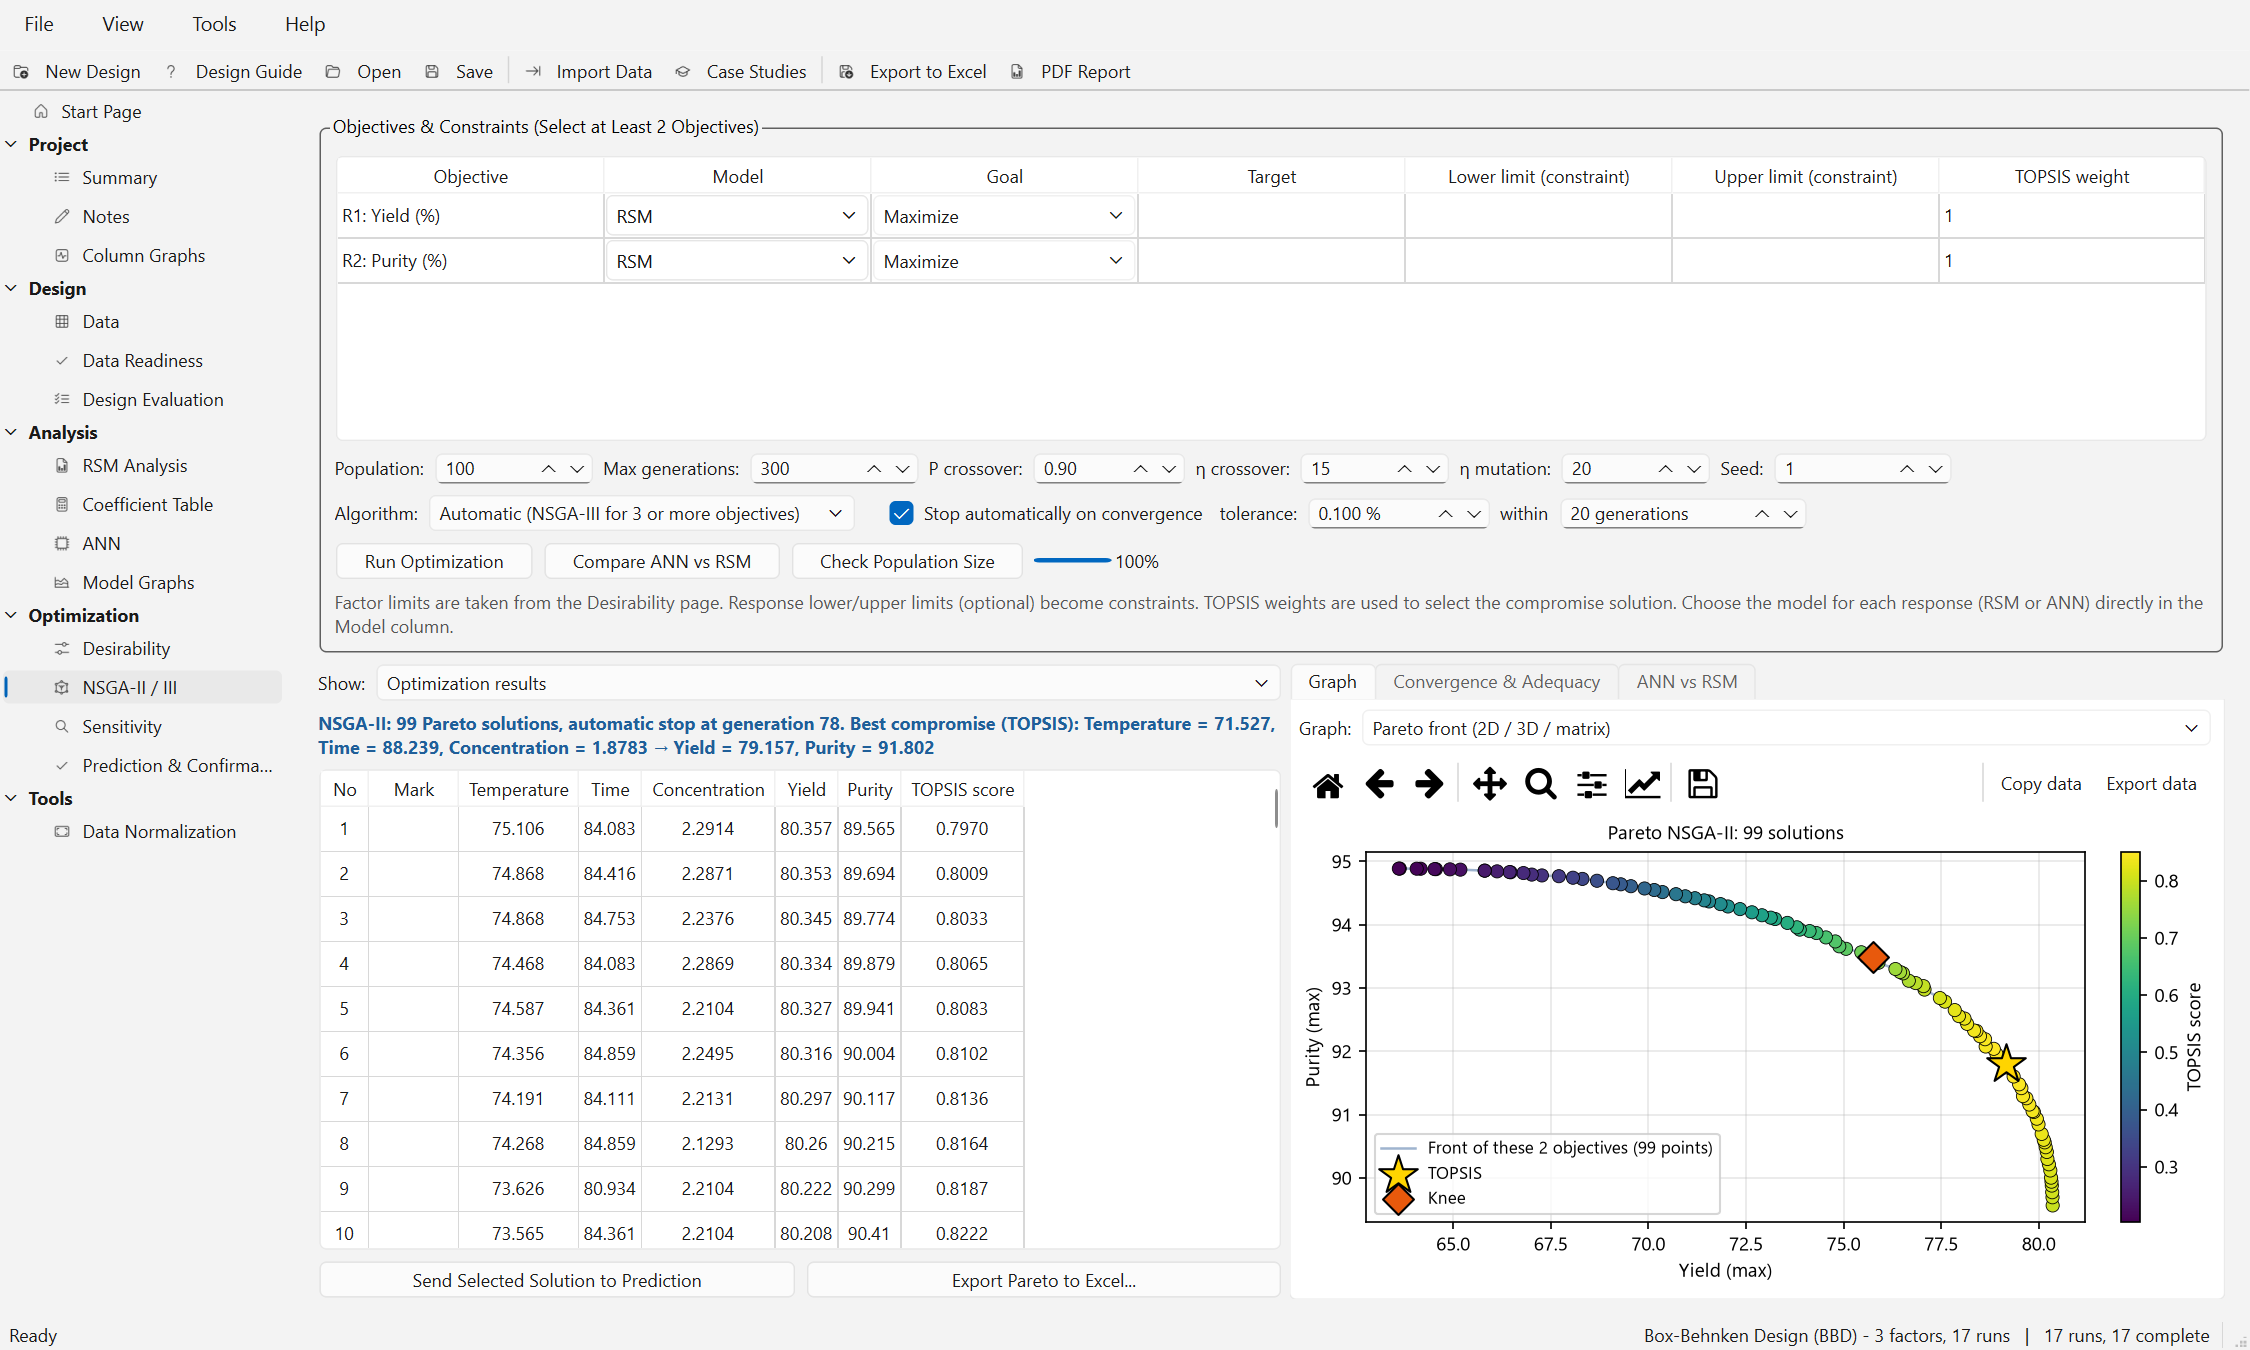
\includegraphics[width=\linewidth]{nsga_front.png}
\caption{NSGA-II front of the BBD case (Yield and Purity maximized, RSM models). Points are colored by TOPSIS score;
star = TOPSIS choice, diamond = knee point.}
\label{fig:ch08-front}
\end{figure}

The front (Figure~\ref{fig:ch08-front}) runs from Purity 94.89 at Yield 63.6 to Purity 89.57 at Yield 80.36: a
clear conflict between the two responses. Along most of the front, Purity falls slowly while Yield rises; above a
Yield of about 78 every further unit of Yield costs much more Purity. The knee lies at the start of this steep part,
and the TOPSIS choice lies inside it because TOPSIS with equal weights values the large Yield range.

\begin{figure}[htbp]
\centering
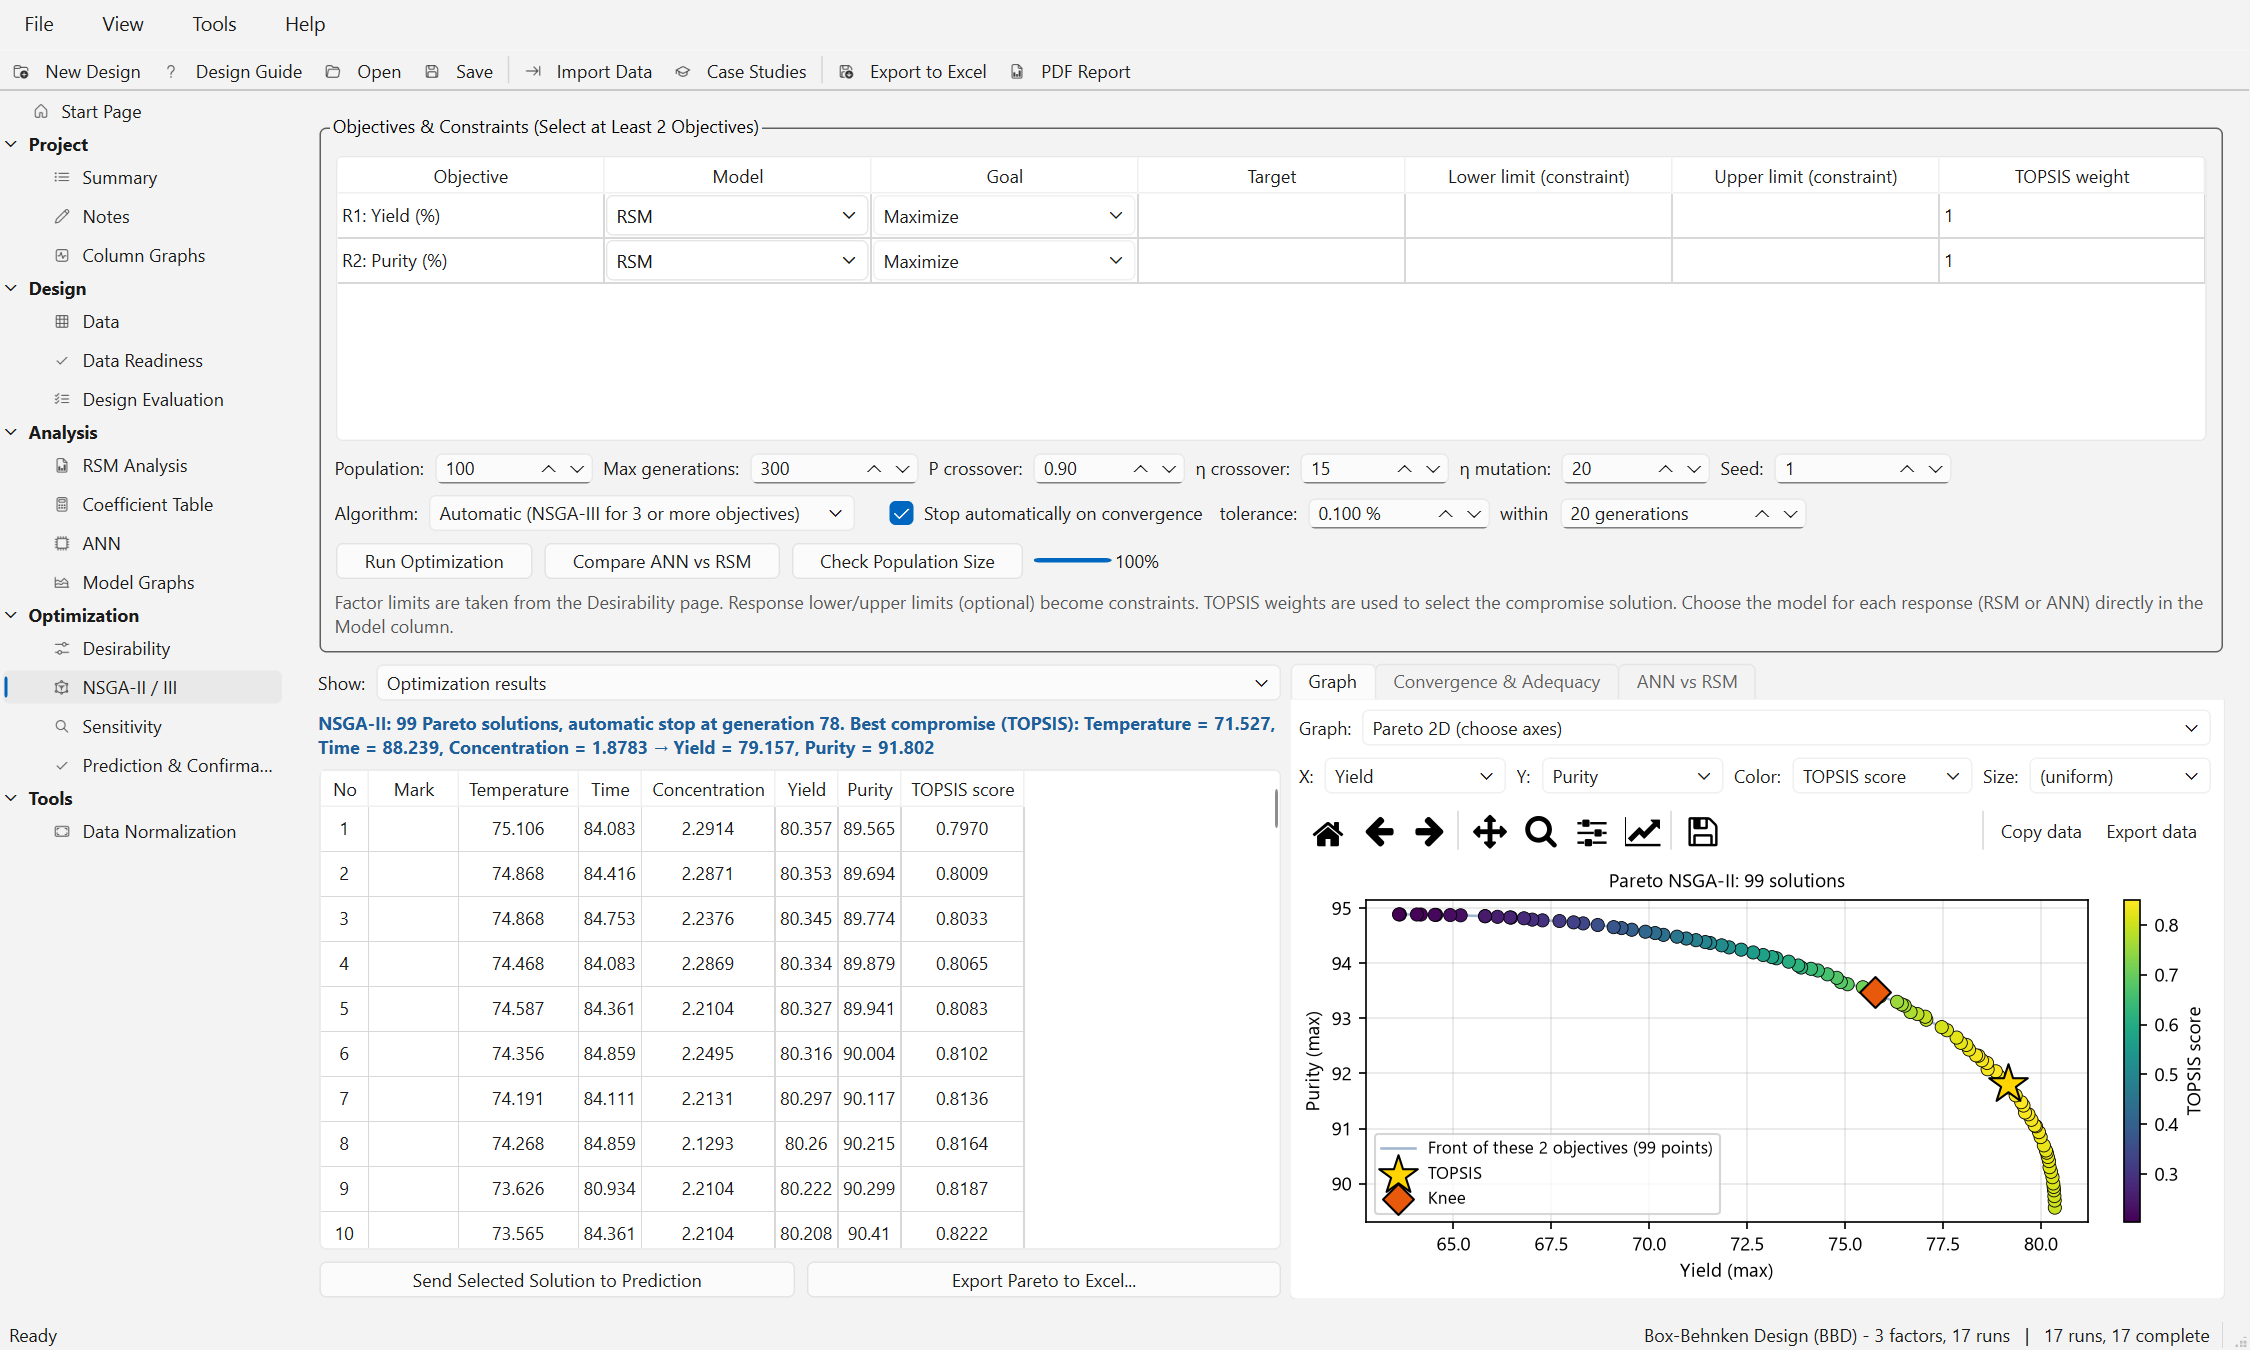
\includegraphics[width=\linewidth]{nsga_front2d.png}
\caption{\ui{Pareto 2D (choose axes)} with the \ui{X:}, \ui{Y:}, \ui{Color:} and \ui{Size:} selectors. With two
objectives it shows the same front as Figure~\ref{fig:ch08-front}.}
\label{fig:ch08-front2d}
\end{figure}

\begin{figure}[htbp]
\centering
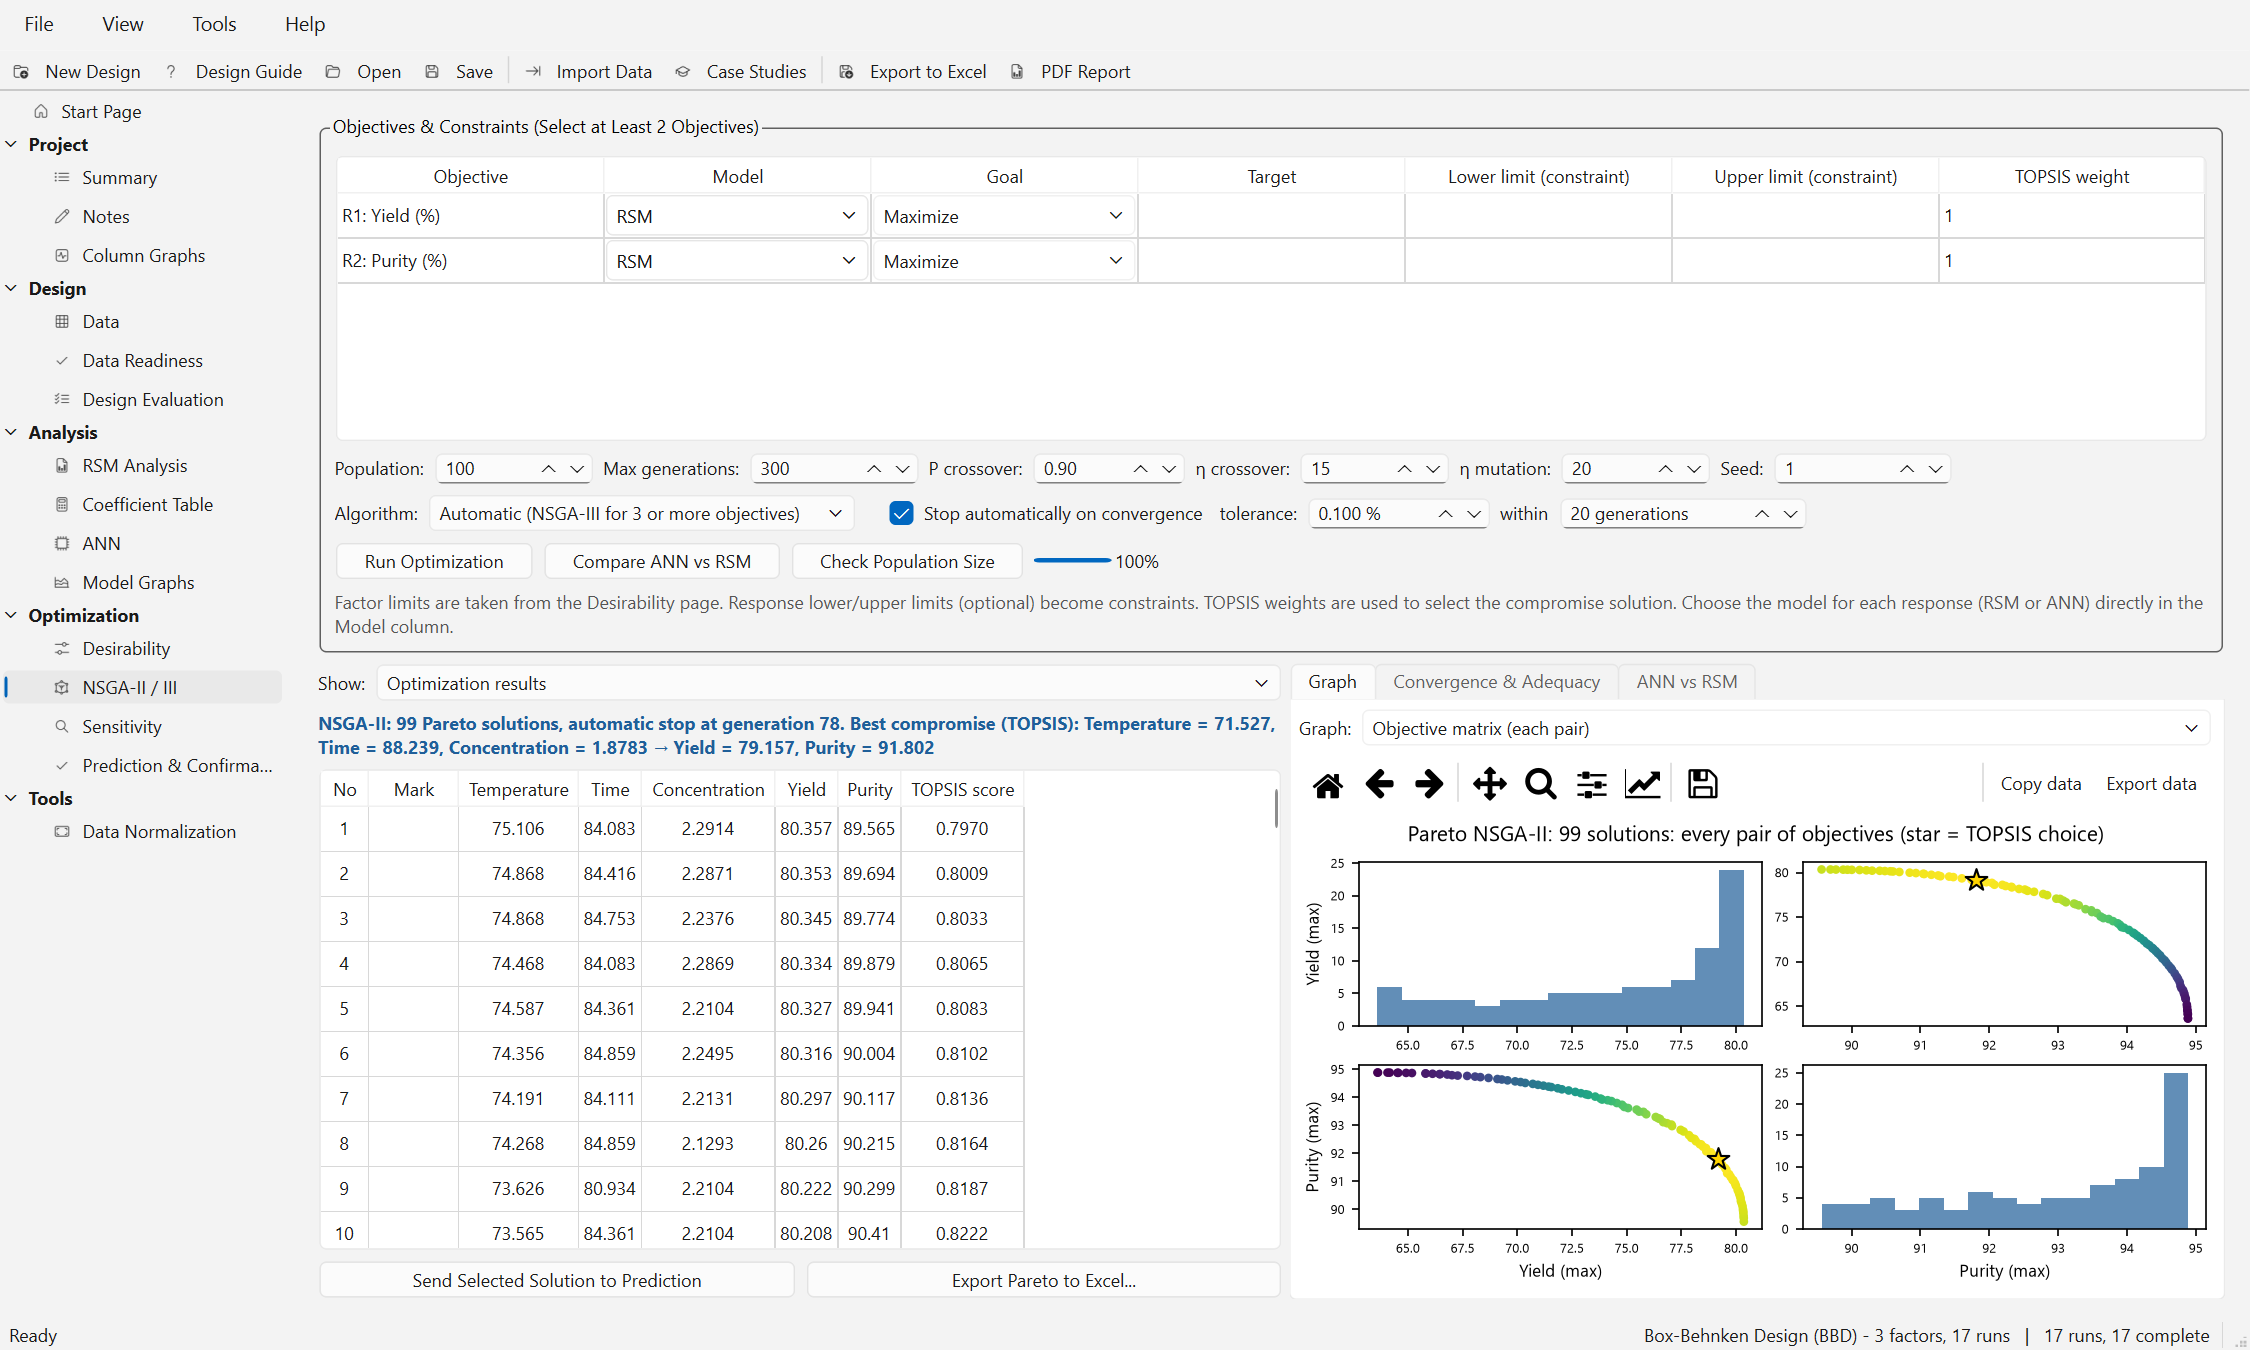
\includegraphics[width=\linewidth]{nsga_matrix.png}
\caption{\ui{Objective matrix (each pair)}: pairwise scatter plots and histograms of the objectives (most useful
for three or more objectives).}
\label{fig:ch08-matrix}
\end{figure}

\begin{figure}[htbp]
\centering
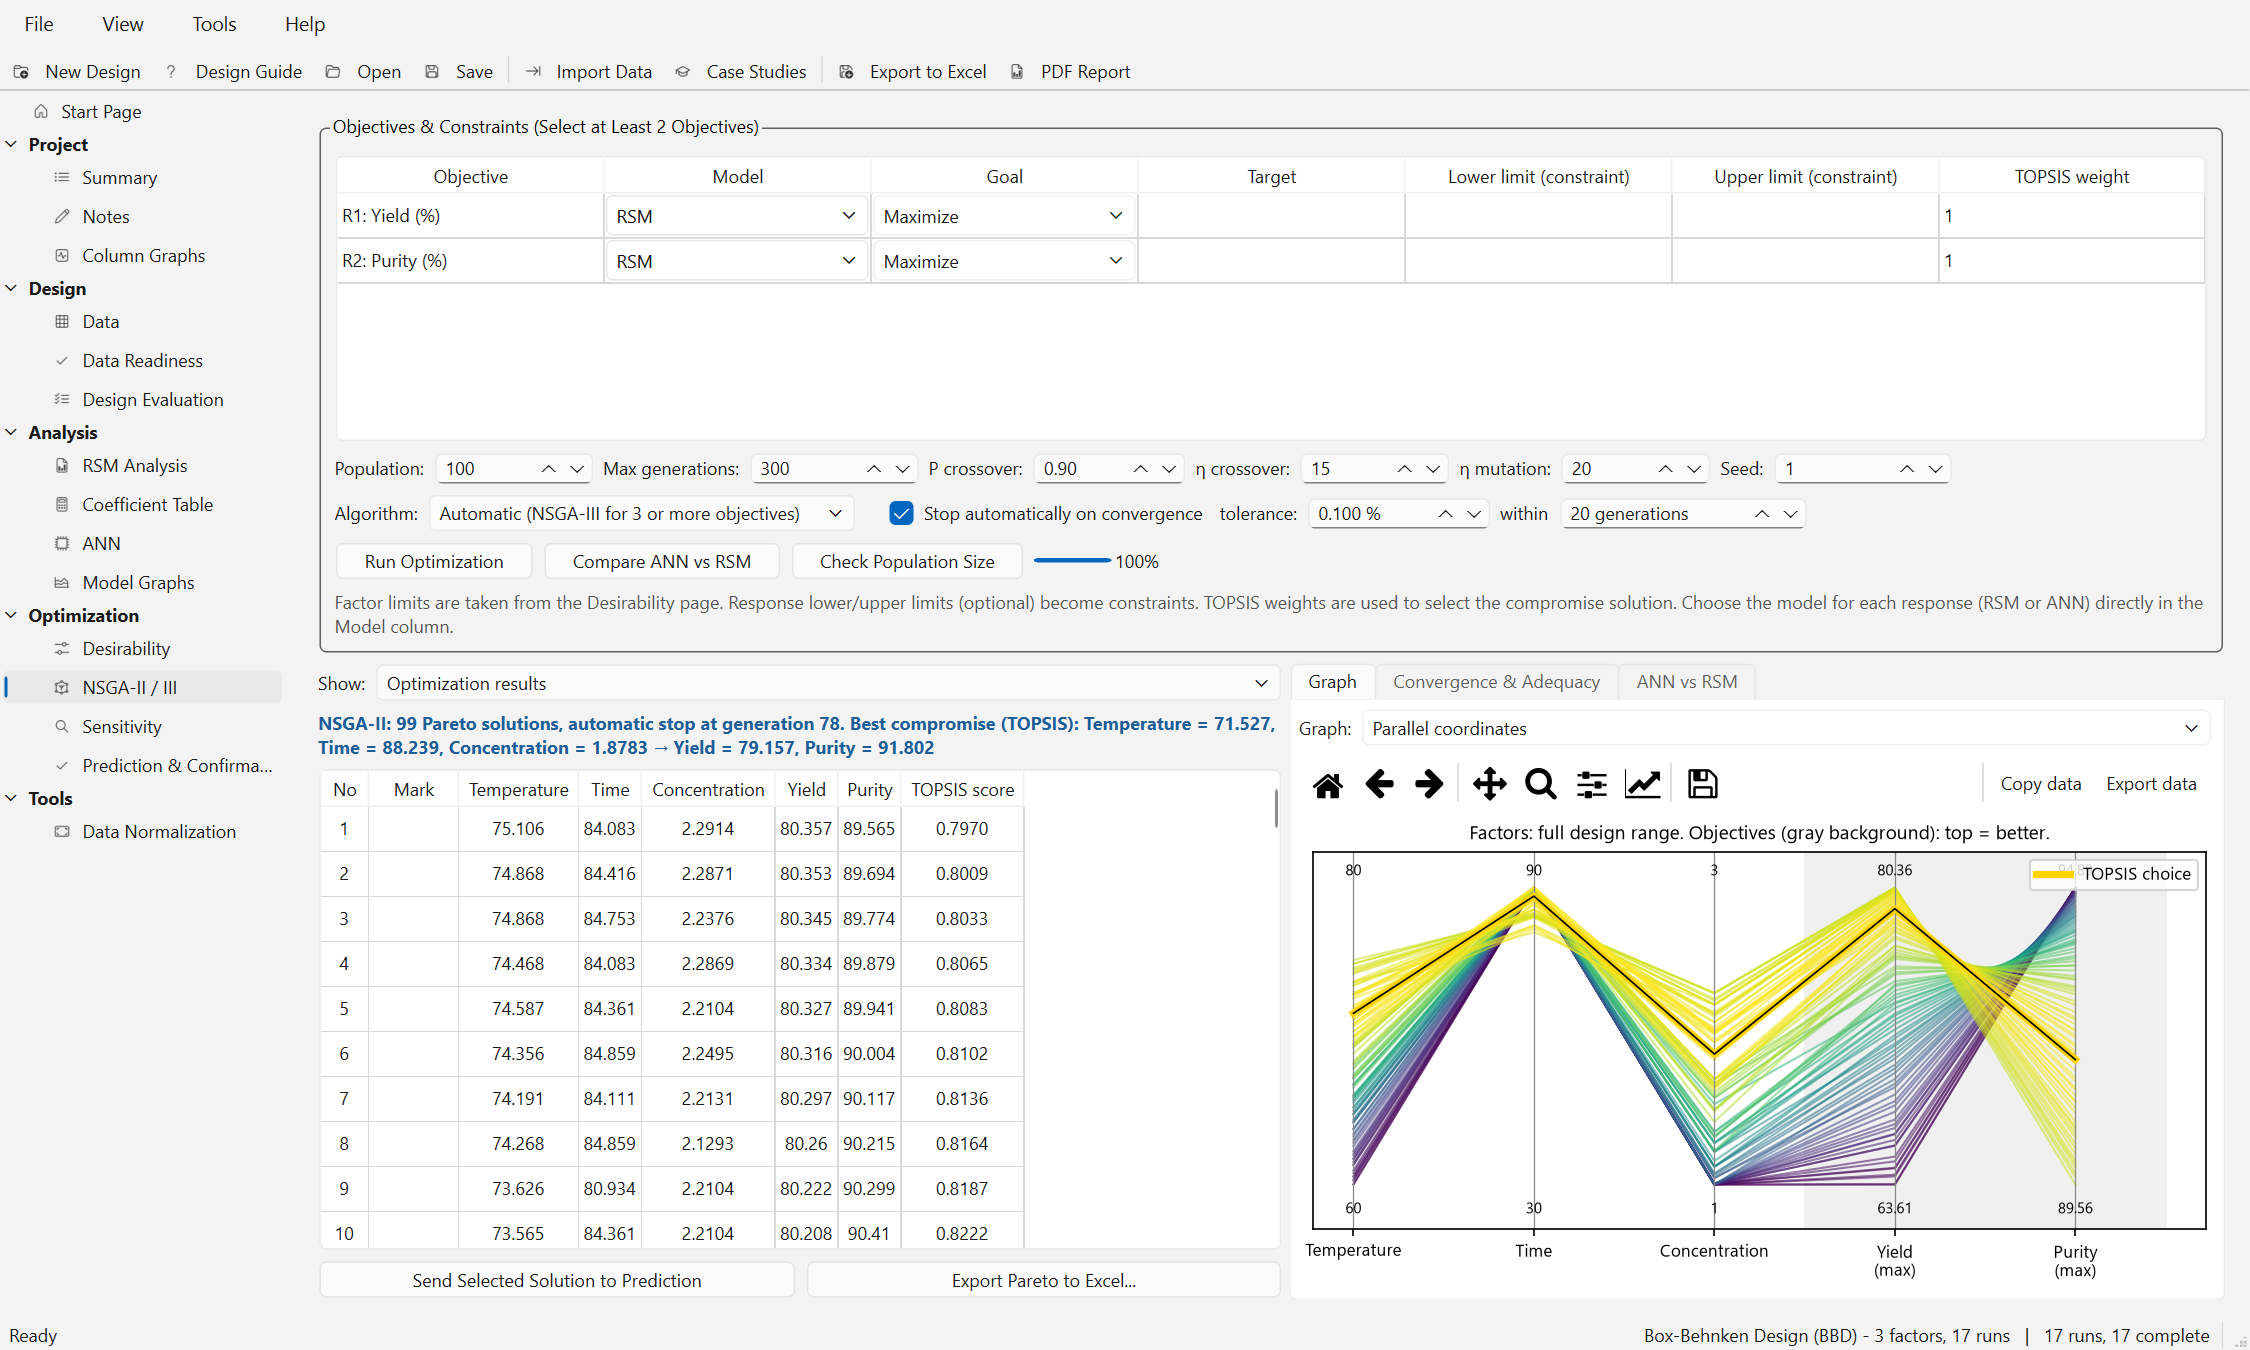
\includegraphics[width=\linewidth]{nsga_parallel.png}
\caption{\ui{Parallel coordinates}: each Pareto solution is a line across the factors (full design range) and the
objectives (grey, top = better); the TOPSIS solution is highlighted.}
\label{fig:ch08-parallel}
\end{figure}

The parallel coordinates (Figure~\ref{fig:ch08-parallel}) show how the front is built: Time stays at or near its upper
limit of 90~min for most solutions (it drops to about 81~min only at the high-Yield end), while Temperature (about 60 to 75~°C) and Concentration (1 to 2.3~\%)
increase together from the high-Purity end to the high-Yield end. Chapter~\ref{chap:9} quantifies this with Spearman
correlations along the front.

\begin{figure}[htbp]
\centering
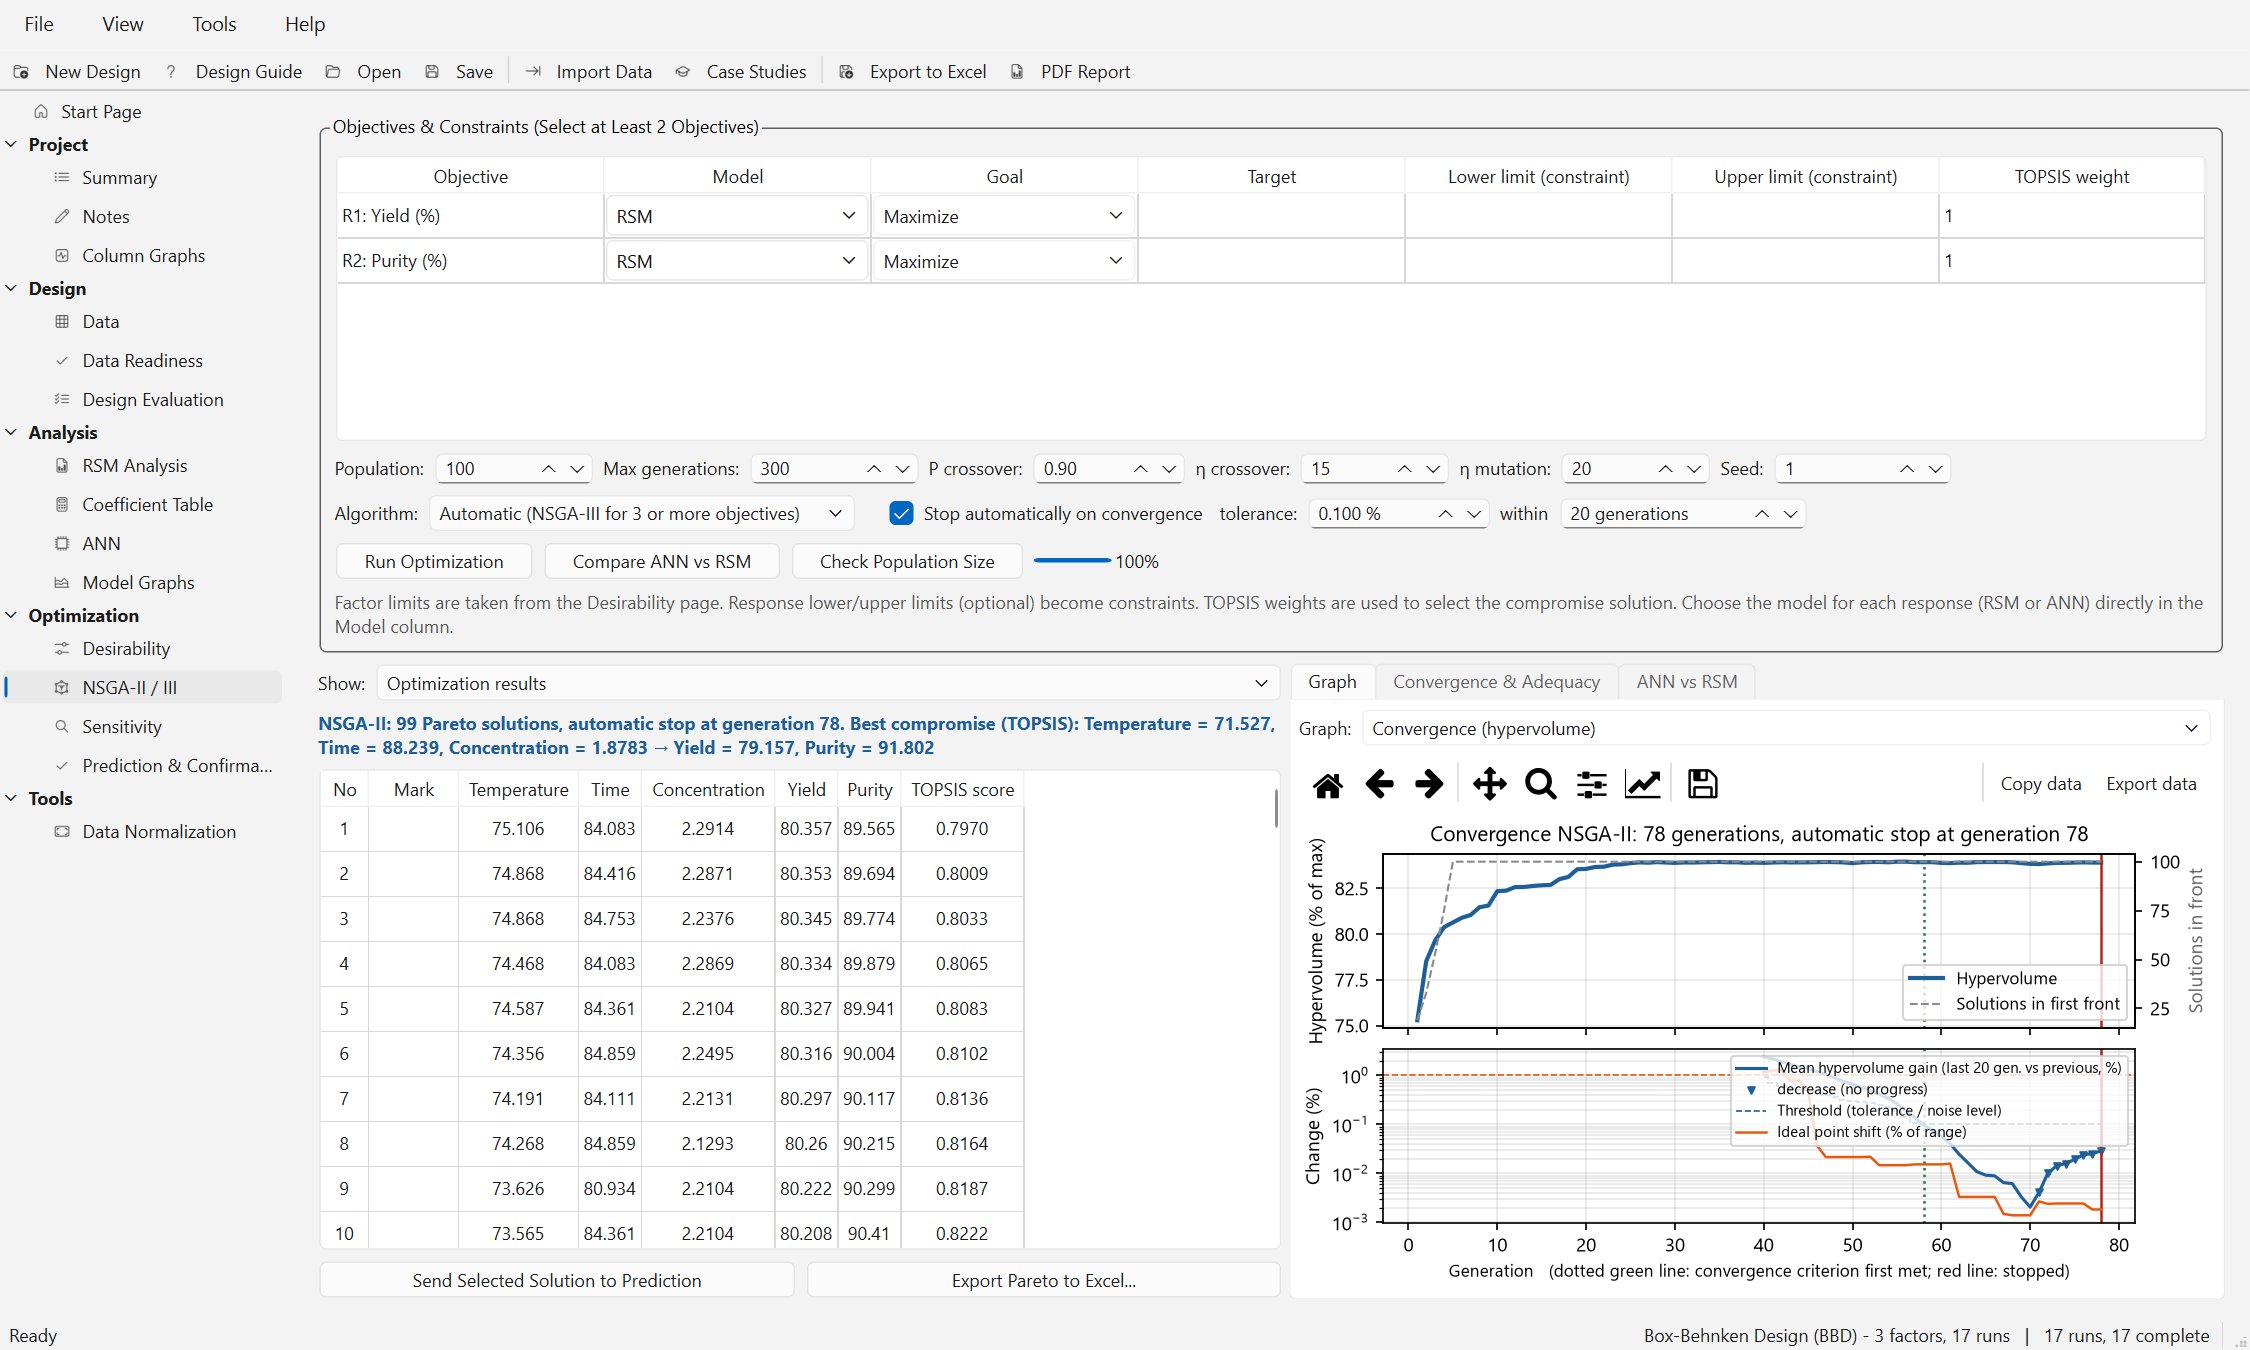
\includegraphics[width=\linewidth]{nsga_convergence.png}
\caption{\ui{Convergence (hypervolume)} of the BBD run: the hypervolume flattens near 84~\% of the maximum; the
criterion is first met at generation 58 (green dotted line) and the run stops at generation 78 (red line).}
\label{fig:ch08-convergence}
\end{figure}

Check~C (Figure~\ref{fig:ch08-convergence}): the hypervolume rises quickly in the first 20 generations and flattens
at 83.9~\% of $1.1^2$. From generation 40 on the gain is compared with the tolerance; the criterion
\eqref{eq:ch08-crit} is first met at generation 58 and holds for the next 20 generations, so the run stops at
generation 78. The report states: \ui{Enough generations: the mean hypervolume of the last 20 generations changed
by only -0.029\% compared with the previous 20 generations (limit 0.10\%) and the ideal point shifted 0.00\% (limit
1\%).} and \ui{All 100 individuals are on the first front (normal for 2 objectives).}

\begin{figure}[htbp]
\centering
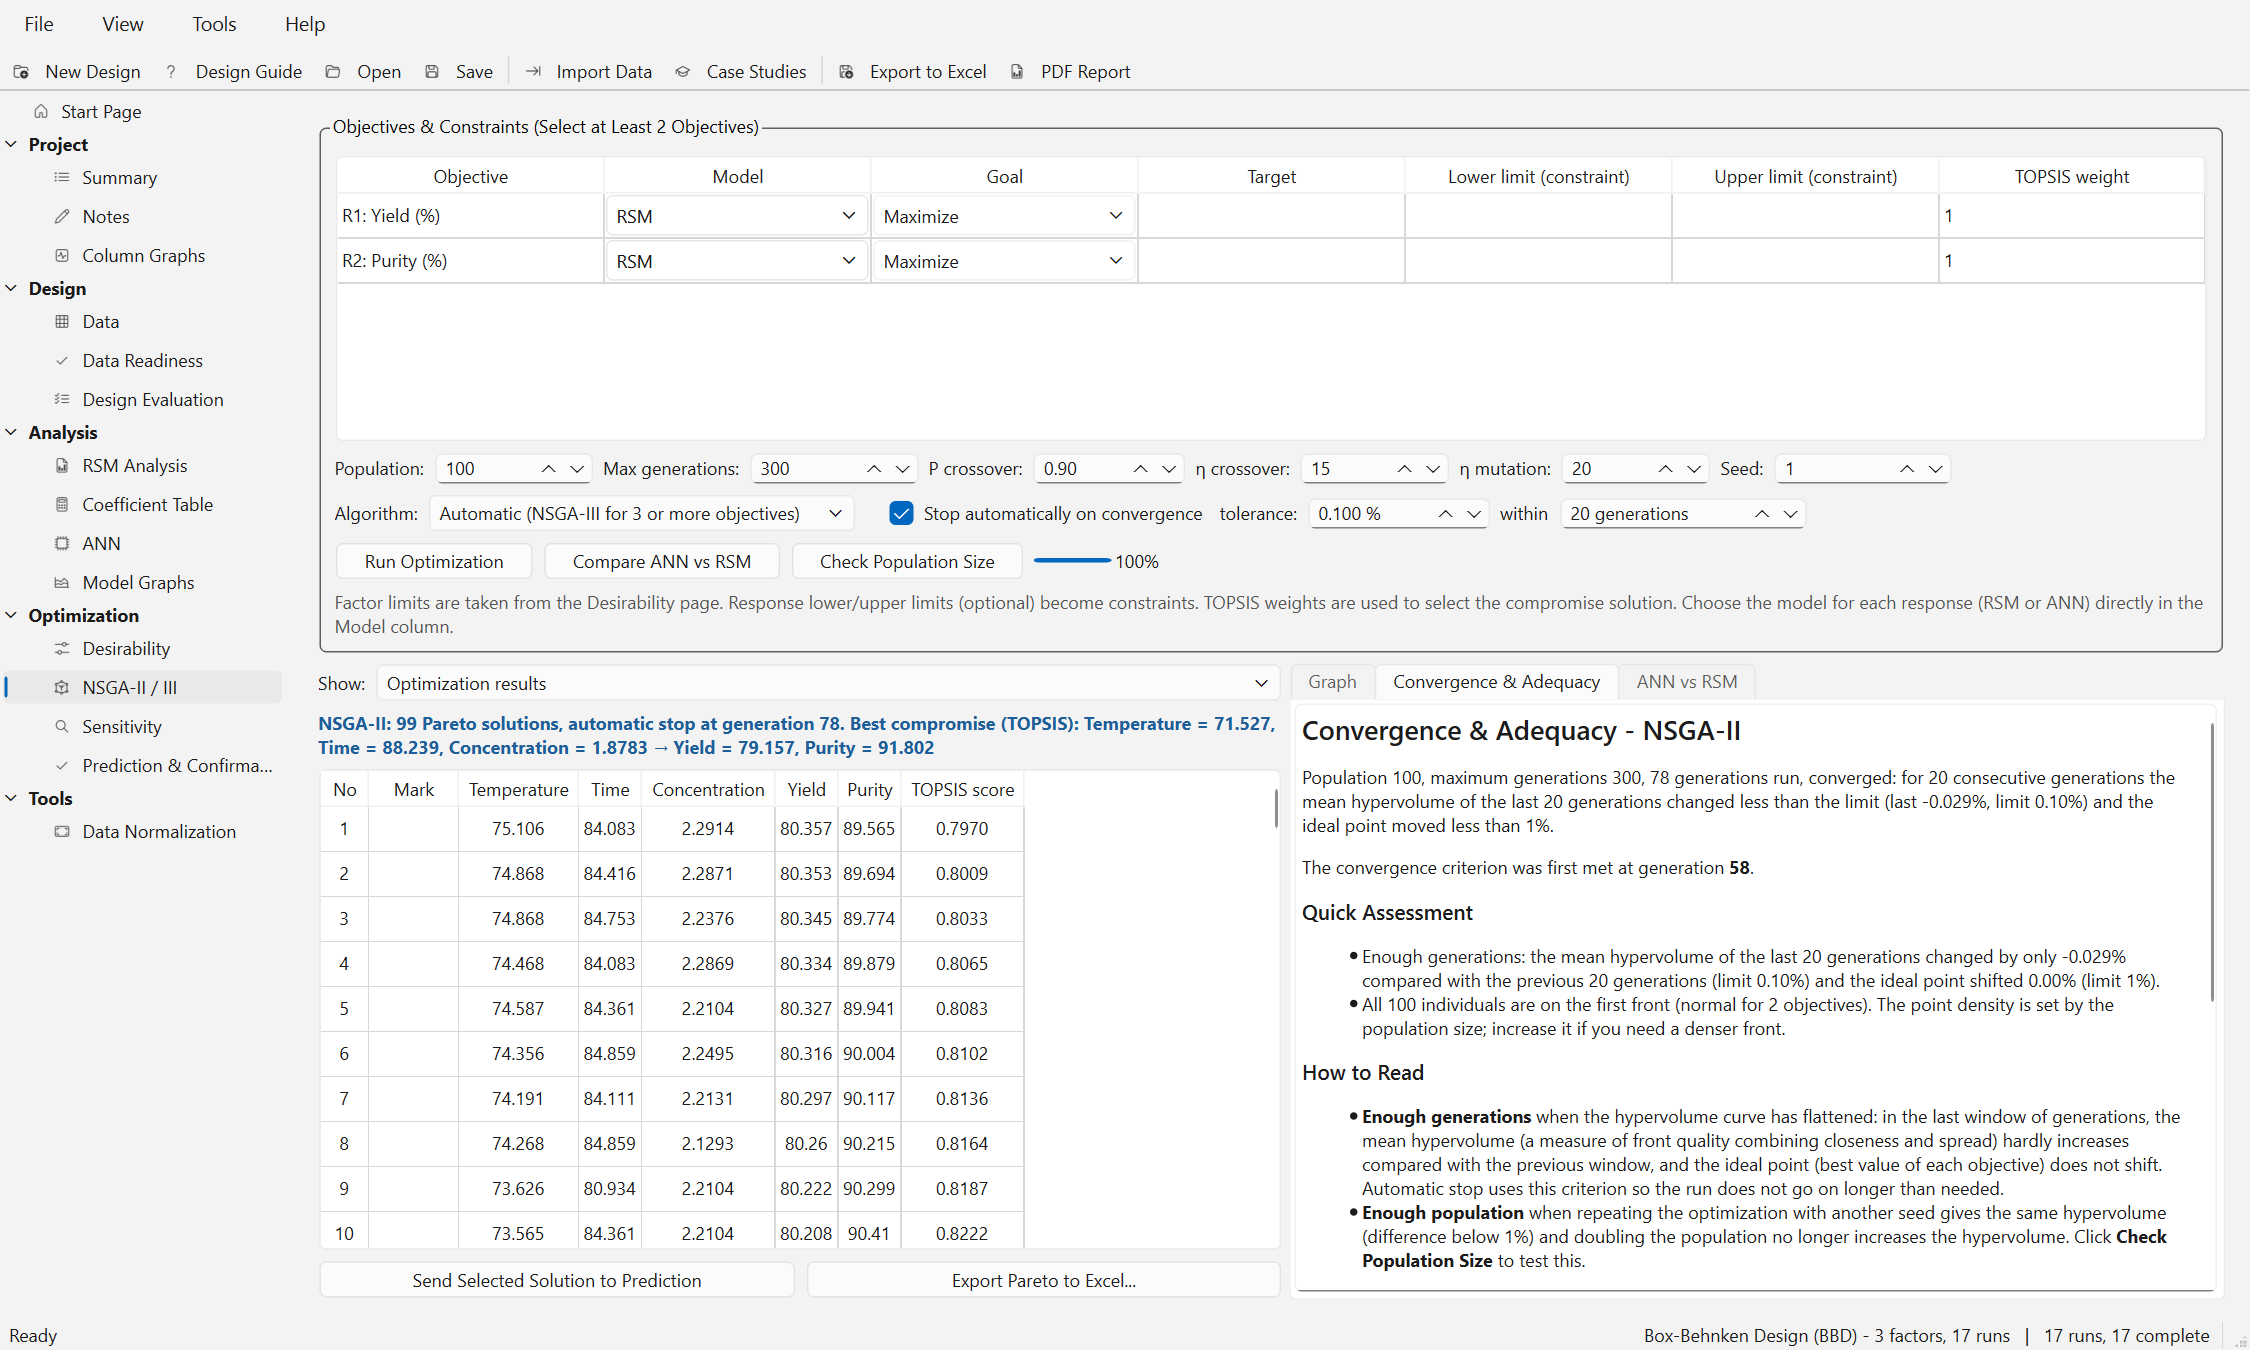
\includegraphics[width=\linewidth]{nsga_population_check.png}
\caption{\ui{Convergence \& Adequacy} tab after \ui{Check Population Size}. The upper part shows the quick
assessment; the table \ui{Adequacy Check Results} follows further down in the report.}
\label{fig:ch08-popcheck}
\end{figure}

\ui{Check Population Size} (Figure~\ref{fig:ch08-popcheck}) gives the results of
Table~\ref{tab:ch08-popcheck}. Another seed changes the hypervolume by at most 0.02~\% and a doubled population adds
0.35~\%, both below 1~\%: \ui{Population: sufficient. Another seed changes the hypervolume by only 0.02\% and a 2x
population adds only 0.35\%.} The TOPSIS choice moves by at most 5.5~\% of a factor range, well below the 15~\%
note. Check~C is therefore passed: the front of this run can be reported.

\begin{table}[htbp]
\centering
\small
\caption{\ui{Adequacy Check Results} for the BBD run (NSGA-II, population 100, seed 1).}
\label{tab:ch08-popcheck}
\begin{tabular}{@{}lrrlrrrr@{}}
\toprule
Run & Pop. & Seed & Generations & Solutions & HV & Diff. & TOPSIS shift (\%) \\
\midrule
Current result & 100 & 1 & 78 (converged) & 99 & 83.93\% & +0.00\% & 0.0 \\
Different seed & 100 & 102 & 70 (converged) & 100 & 83.93\% & +0.01\% & 5.5 \\
Different seed 2 & 100 & 203 & 81 (converged) & 100 & 83.94\% & +0.02\% & 2.2 \\
Population 2x & 200 & 1 & 67 (converged) & 195 & 84.22\% & +0.35\% & 2.9 \\
\bottomrule
\end{tabular}
\end{table}

\textbf{When check C fails.} If the quick assessment says \ui{Not enough generations yet}, increase \ui{Max
generations} (the automatic stop still ends the run when it converges). If the population check is not passed,
double the population and check again. With three or more objectives a saturated first front (all $N$ members
non-dominated) is a hint that the population is too small to describe the front. In the three-objective POE example
above the noise level raised the threshold \eqref{eq:ch08-tau} from 0.10~\% to 0.25~\%, and the quick assessment
recommended \ui{try 2x the population and compare}.

% ======================================================================================================
\section{Check D: ANN versus RSM fronts}
\label{sec:ch08-checkD}

\subsection{Purpose}
An optimum found on a model is only as good as the model. When both an RSM and an ANN model are available, check~D
asks whether the optimization result depends on the choice of model. If the two models predict similar values on
the Pareto solutions and lead to similar compromise settings, the result is robust. If they disagree, the
disagreement marks the region where the data do not determine the response well enough, the same idea used to
locate uncertain regions with disagreeing networks \citep{krogh1995}. Confirmation runs are then needed at both
candidate settings.

\subsection{How to use}
\begin{enumerate}
  \item Train an ANN for the objective responses on the ANN page, preferably with \ui{Optimize All Responses (One
        Click)} so that each network is selected by cross-validation (check~A, Chapter~\ref{chap:7}). Without any ANN the button
        answers \ui{There is no ANN model for the objective responses yet. Train an ANN first on the ANN page
        (Optimize All Responses button).}
  \item Set the objectives as for a normal run and click \ui{Compare ANN vs RSM}. The progress text shows
        \ui{[1/2] RSM: \dots} and \ui{[2/2] ANN: \dots}.
  \item Read the \ui{ANN vs RSM} tab and the three comparison graphs. With \ui{Show:} you can inspect each front in
        the solutions table.
\end{enumerate}

\subsection{Theory as implemented}
\begin{enumerate}
  \item The optimization is run twice with identical settings: once with RSM for every objective and once with ANN
        for every objective. A response without an ANN keeps its RSM model on the ANN front (warning \ui{No ANN yet
        for \dots; on the ANN front these responses still use RSM.}).
  \item \textbf{Cross-prediction.} The solutions of each front are predicted with the other model, giving
        $y^\text{self}$ and $y^\text{other}$ for every solution of both fronts.
  \item \textbf{Hypervolume.} The four objective sets (RSM front by RSM, RSM front by ANN, ANN front by ANN, ANN
        front by RSM) are normalized jointly, and $HV_{(\text{front, assessor})}$ is computed as in check~C (in \%
        of $1.1^m$).
  \item \textbf{Prediction difference.} For each objective $o$, over the solutions of both fronts,
        \begin{equation}
        \Delta_o^\text{mean}=\frac{100}{R_o}\operatorname{mean}\bigl|y^\text{self}-y^\text{other}\bigr|,\qquad
        \Delta_o^\text{max}=\frac{100}{R_o}\max\bigl|y^\text{self}-y^\text{other}\bigr|,
        \label{eq:ch08-delta}
        \end{equation}
        where $R_o$ is the range (maximum minus minimum) of the response data; for a POE objective it is the range
        of all predicted POE values. The decisive value is the worst objective,
        $\Delta=\max_o\Delta_o^\text{mean}$.
  \item \textbf{Distance between the compromise choices.} With $\mathbf x^\text{RSM}$ and $\mathbf x^\text{ANN}$ the
        TOPSIS solutions of the two fronts (coded units) and $[l_j,u_j]$ the coded design range,
        \begin{equation}
        dx=100\,\max_j\frac{|x^\text{RSM}_j-x^\text{ANN}_j|}{u_j-l_j}.
        \label{eq:ch08-dx}
        \end{equation}
  \item \textbf{Model quality} per objective: RSM predicted $R^2$, ANN test $R^2$ of the final model's single
        split, and ANN cross-validation $Q^2$ from the architecture search (if one was run).
\end{enumerate}

\subsection{Conclusion rules and messages}
\begin{table}[htbp]
\centering
\small
\caption{Verdict of check~D ($\Delta$ in \% of the response range, $dx$ in \% of the factor range).}
\label{tab:ch08-checkD}
\begin{tabularx}{\linewidth}{@{}>{\raggedright\arraybackslash}p{2.4cm} >{\raggedright\arraybackslash}p{3.2cm} >{\raggedright\arraybackslash}X@{}}
\toprule
Verdict & Condition & Message (beginning) and action \\
\midrule
Agree (green) & $\Delta<5$ and $dx<15$ & \ui{Both models agree: predictions on the front differ by only \dots\ The
optimization result does not depend on the choice of model.} \\
Partial (amber) & $\Delta<10$, not ``agree'' & \ui{The models agree only partly.} followed by the criterion that
failed: both (\ui{Make confirmation runs at both TOPSIS points.}), only $\Delta$ (\ui{Check the region where the
differences are largest before relying on the front there.}) or only $dx$ (\ui{The front is flat in that region:
several settings give similar results.}). \\
Differ (red) & $\Delta\ge10$ & \ui{The models differ considerably: \dots\ Do not rely on just one model: make
confirmation runs at both TOPSIS points.} The $dx$ part states whether it is within or above 15~\%. \\
\bottomrule
\end{tabularx}
\end{table}
The thresholds are 5~\% and 10~\% for $\Delta$ and 15~\% for $dx$. They are practical rules: a mean difference of
5~\% of the observed range is of the order of the prediction error of a good response surface model, and 15~\% of a
factor range is a distance at which two settings are clearly different experiments.

Further bullets of the conclusion:
\begin{itemize}
  \item \ui{According to each model, the ANN|RSM front promises a better trade-off (hypervolume $x$\% vs $y$\%).}
        compares $HV_{(\text{RSM,RSM})}$ with $HV_{(\text{ANN,ANN})}$.
  \item If a front loses more than 5 percentage points of hypervolume when assessed by the other model:
        \ui{The \dots\ front loses a lot of hypervolume when assessed by the other model. Its advantage may exist
        only in the \dots\ model (for example, ANN extrapolating or RSM being too simple).}
  \item \ui{Prediction accuracy on new data: RSM mean Pred R² \dots, ANN mean cross-validation Q² \dots. If the
        fronts differ, the model with higher accuracy is more trustworthy.} The ANN value is the mean
        cross-validation $Q^2$ of the architecture search when every objective has an ANN found by a search; it is
        more reliable than one train/test split of a small data set. Otherwise the bullet falls back to
        \ui{ANN mean test R² (single split)}, which for small data sets rests on very few runs; compare it with the
        \ui{Model Quality per Response} table.
\end{itemize}

\subsection{Report and plots}
The \ui{ANN vs RSM} tab contains the sections \ui{Pareto Front Comparison: ANN vs RSM}, \ui{Model Quality per
Response}, \ui{Front Size} (Pareto solutions, generations run, \ui{Hypervolume, assessed by own model} and
\ui{Hypervolume, assessed by other model}), \ui{Prediction Difference on Pareto Solutions} ($\Delta^\text{mean}$ and
$\Delta^\text{max}$), \ui{TOPSIS Compromise Solutions} (both choices with factor values and predictions of both
models, and $dx$) and \ui{Conclusion}. The graphs are:
\begin{description}[style=nextline]
  \item[\ui{ANN vs RSM: 2D front}] Both fronts on the chosen \ui{X:} and \ui{Y:} axes (RSM blue circles, ANN orange
        triangles). Filled stars are the TOPSIS choices; hollow stars are the same choices predicted by the other
        model, connected by dashed arrows. A long arrow means the other model disagrees about that setting.
  \item[\ui{ANN vs RSM: cross-prediction}] One panel per objective: RSM prediction against ANN prediction for the
        solutions of both fronts, with the 1:1 line; the panel title gives $\Delta^\text{mean}$.
  \item[\ui{ANN vs RSM: factors}] Parallel coordinates of the factor settings of both fronts over the full design
        range, with thick lines for the two TOPSIS choices.
\end{description}

\subsection{Example: BBD extraction}
\label{sec:ch08-checkD-example}
For the BBD case the ANNs were selected with \ui{Optimize All Responses (One Click)} (default search settings,
1 CPU core, seed 1): 3-4-1 for Yield (cross-validation $Q^2=0.624$) and 3-5-1 for Purity ($Q^2=0.774$), both
\ui{Good fit}. \ui{Compare ANN vs RSM} with the settings of Section~\ref{sec:ch08-nsga-example} gives
Figures~\ref{fig:ch08-cmp-front}--\ref{fig:ch08-cmp-report}.

\begin{figure}[htbp]
\centering
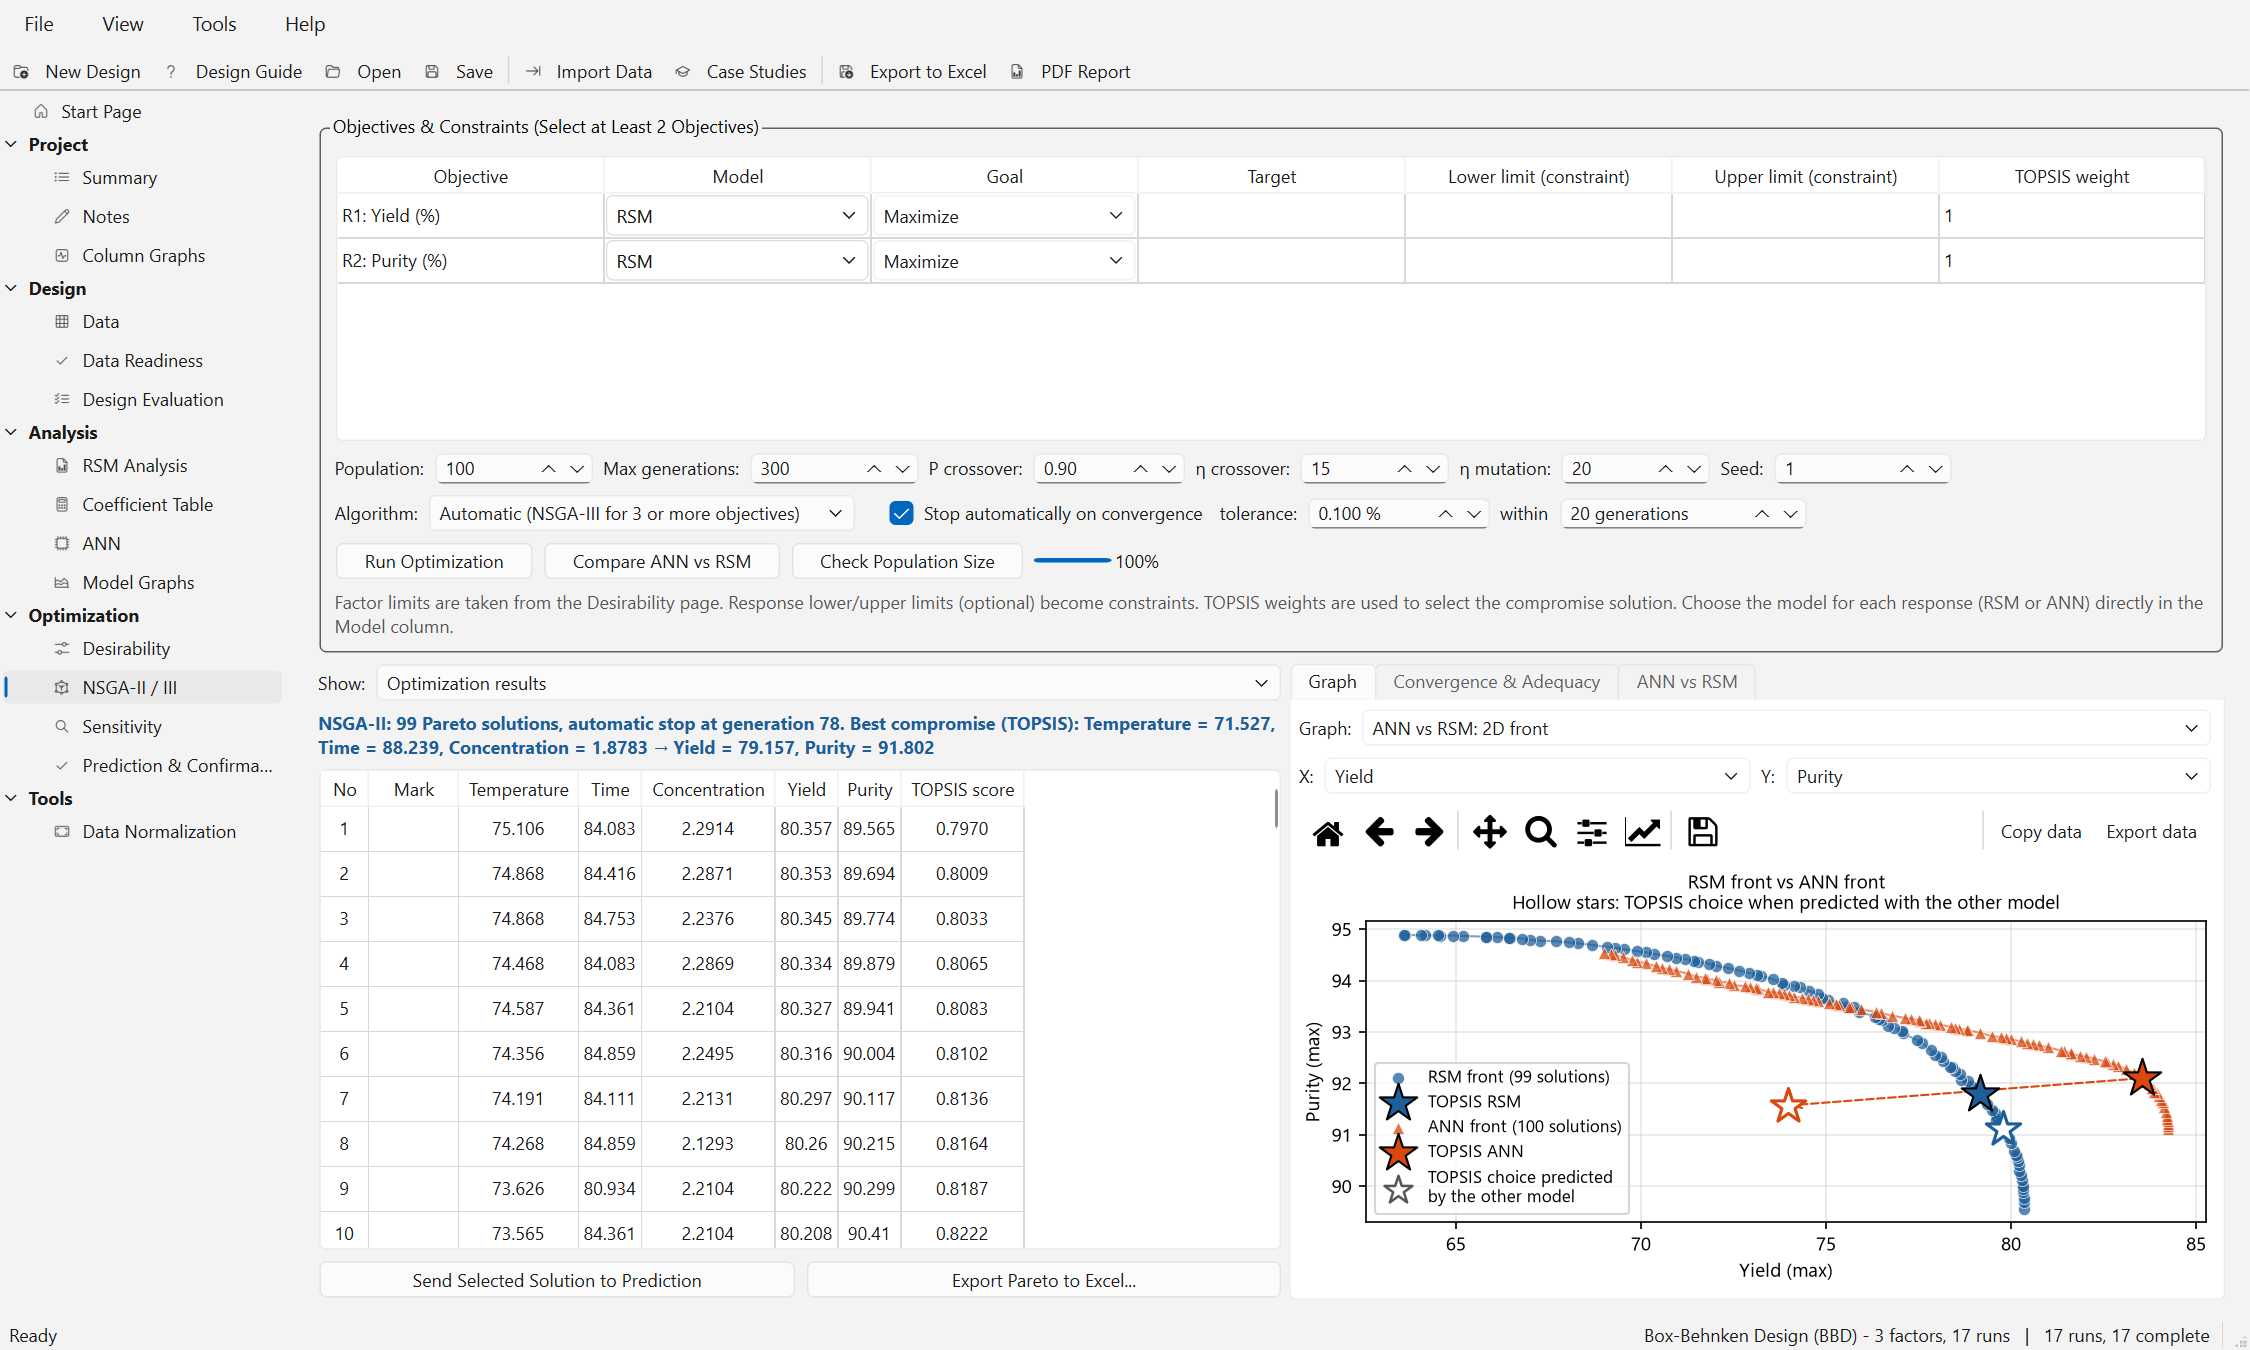
\includegraphics[width=\linewidth]{nsga_compare_front.png}
\caption{\ui{ANN vs RSM: 2D front}: RSM front (blue, 99 solutions) and ANN front (orange, 100 solutions). Hollow stars:
each TOPSIS choice predicted by the other model.}
\label{fig:ch08-cmp-front}
\end{figure}

\begin{figure}[htbp]
\centering
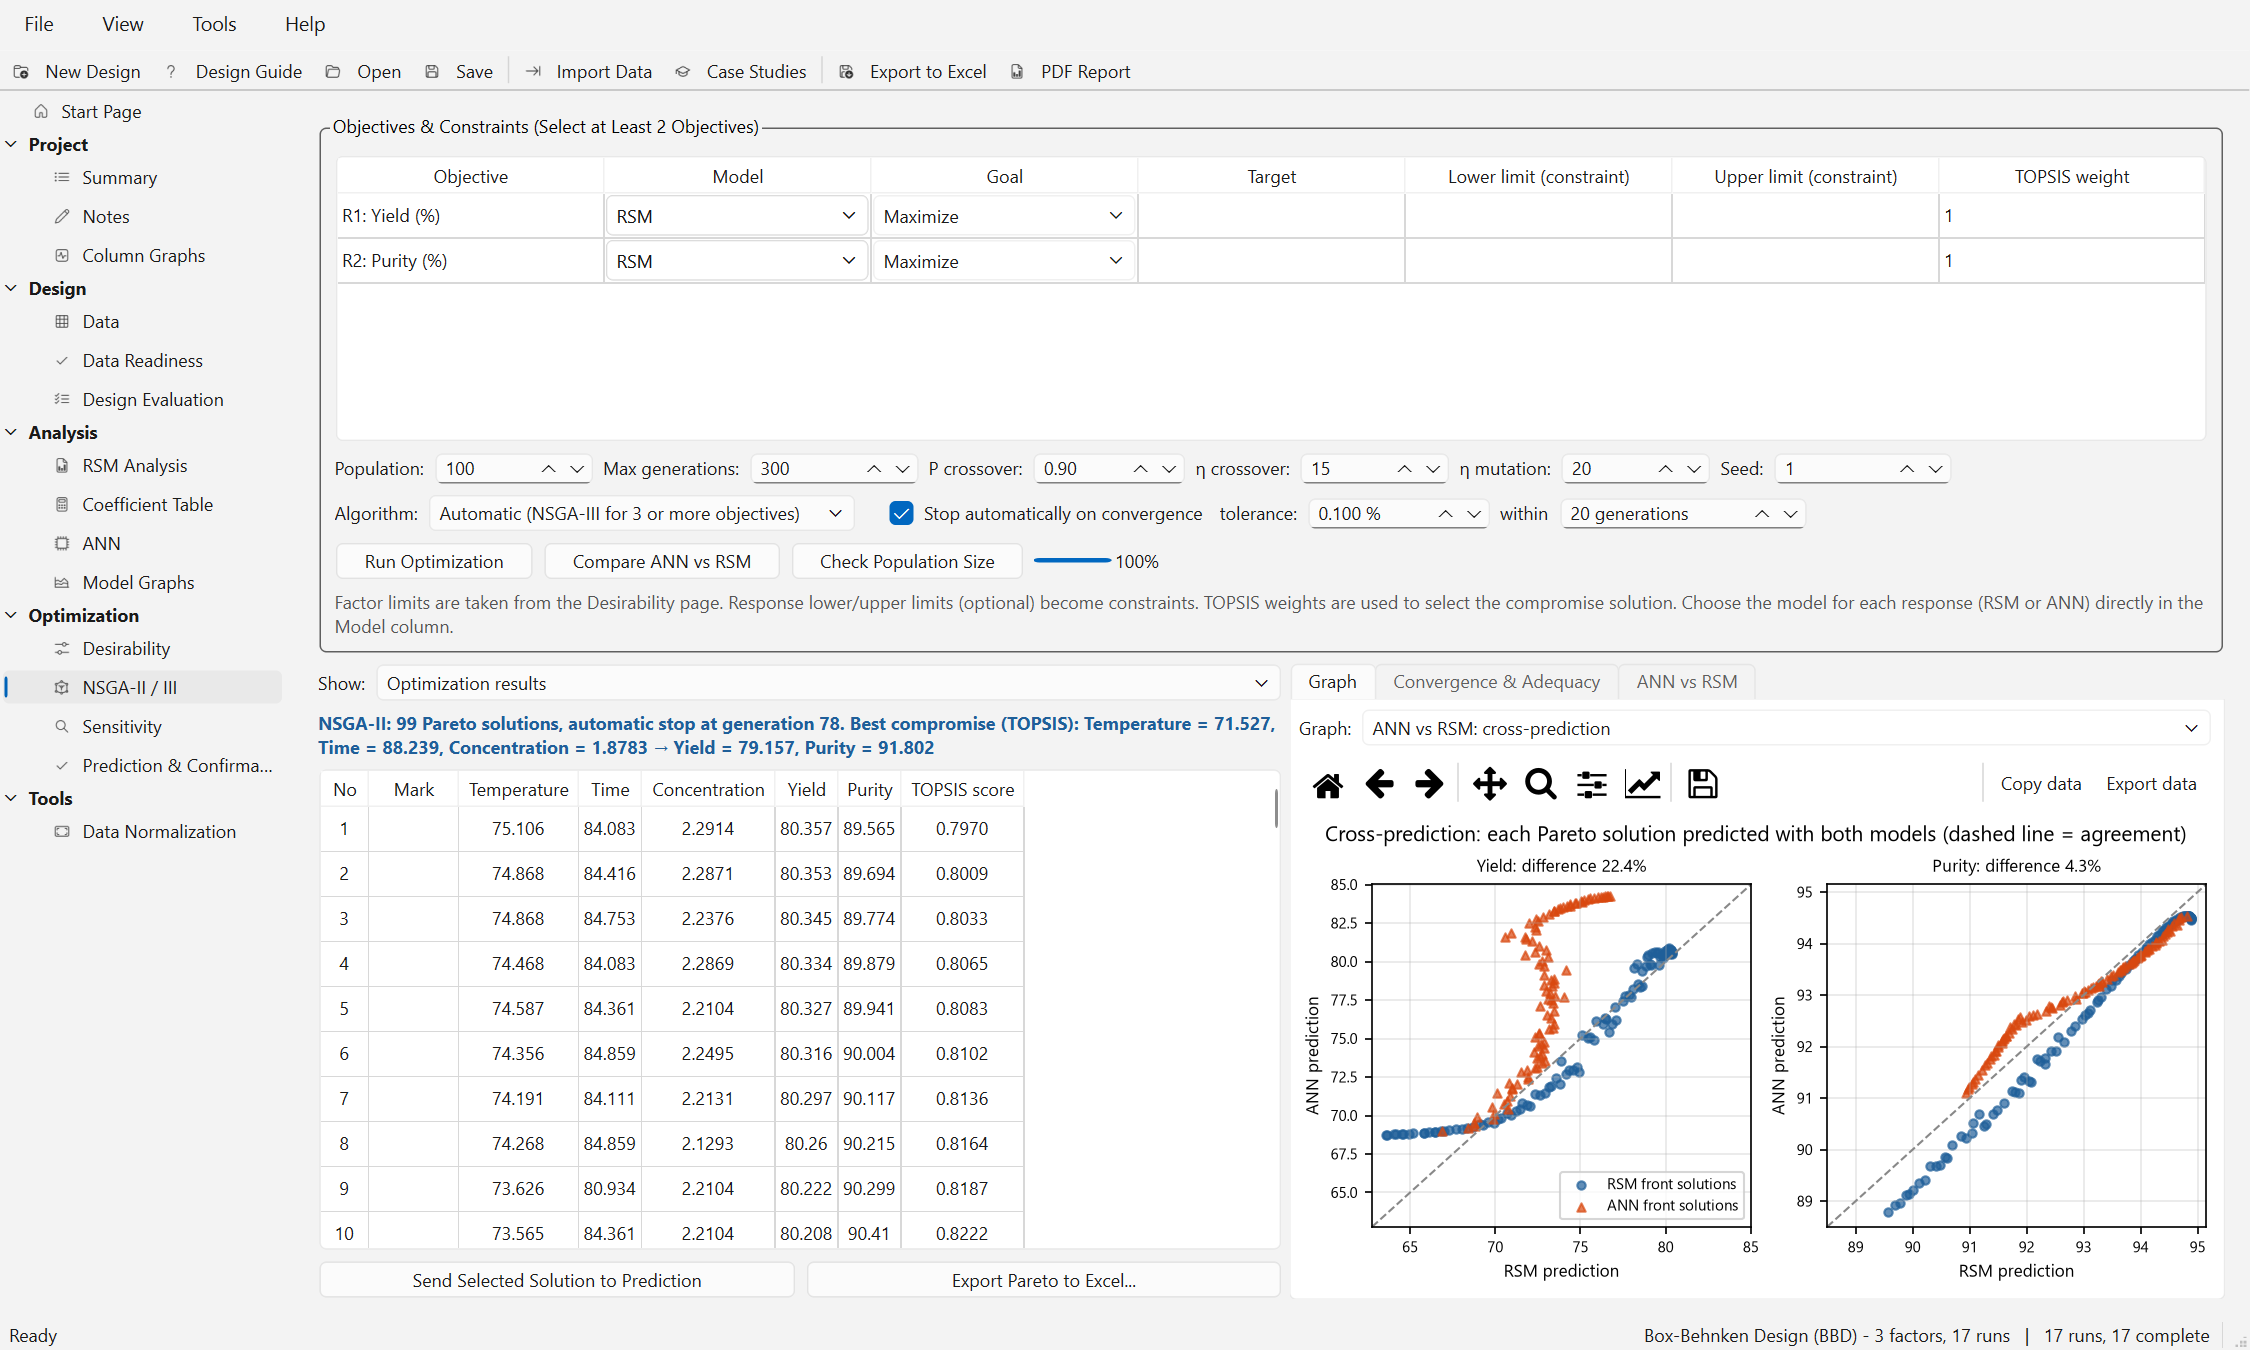
\includegraphics[width=\linewidth]{nsga_compare_cross.png}
\caption{\ui{ANN vs RSM: cross-prediction}: Yield differs by 22.4~\% of its data range on average, Purity by
4.3~\%.}
\label{fig:ch08-cmp-cross}
\end{figure}

\begin{figure}[htbp]
\centering
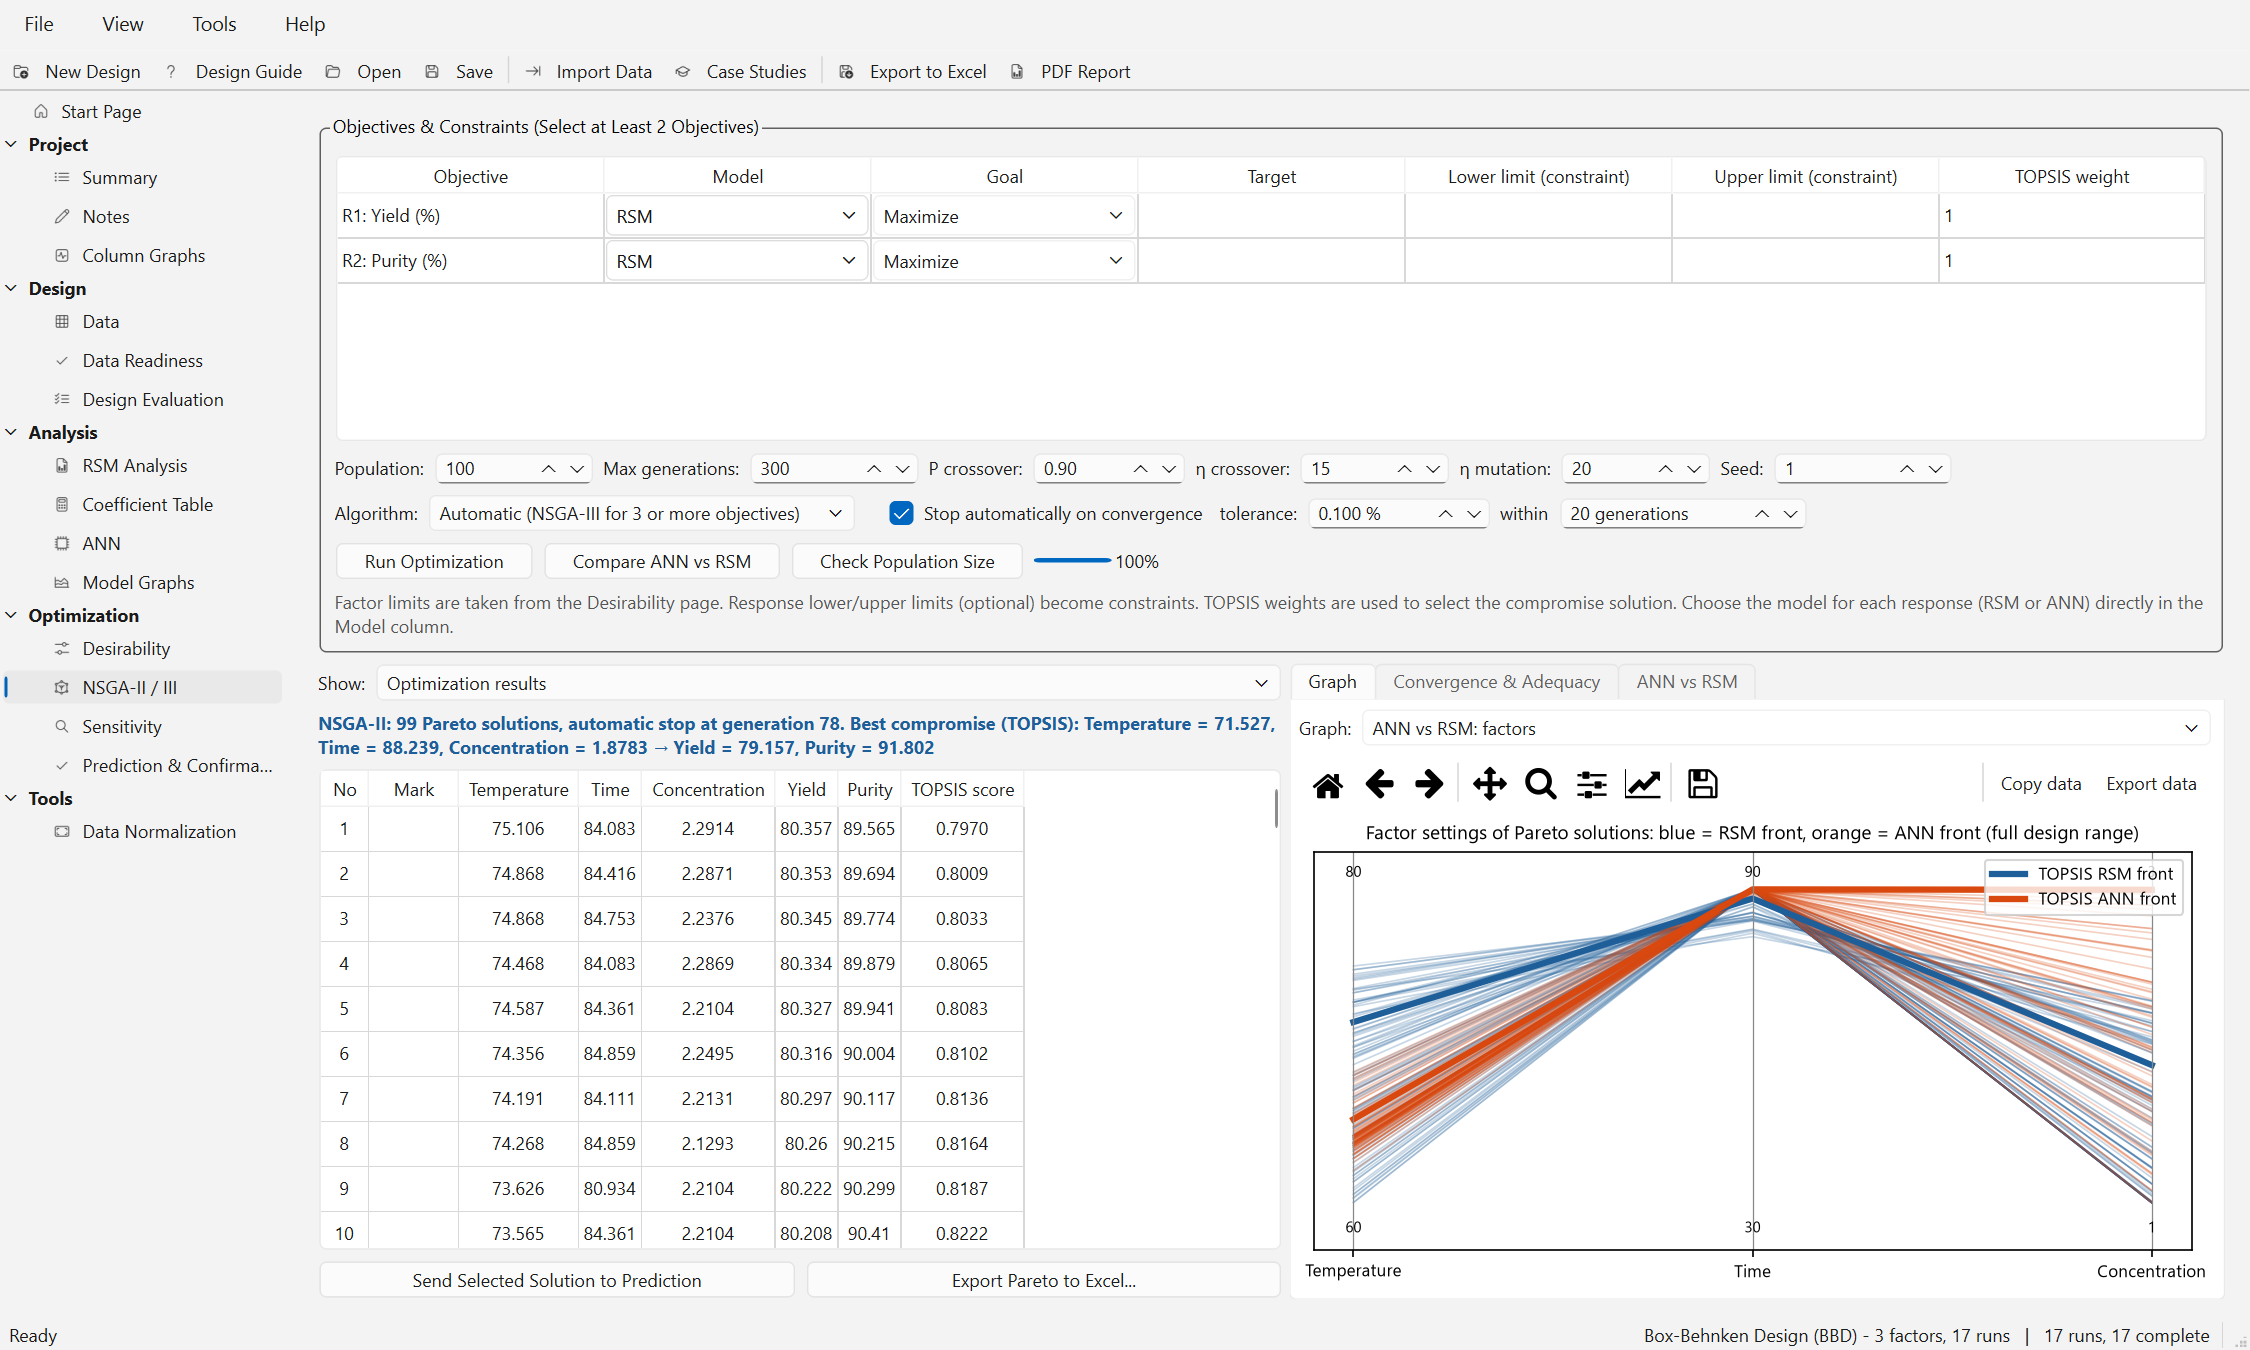
\includegraphics[width=\linewidth]{nsga_compare_factors.png}
\caption{\ui{ANN vs RSM: factors}: the ANN front prefers lower Temperature and higher Concentration than the RSM
front.}
\label{fig:ch08-cmp-factors}
\end{figure}

\begin{figure}[htbp]
\centering
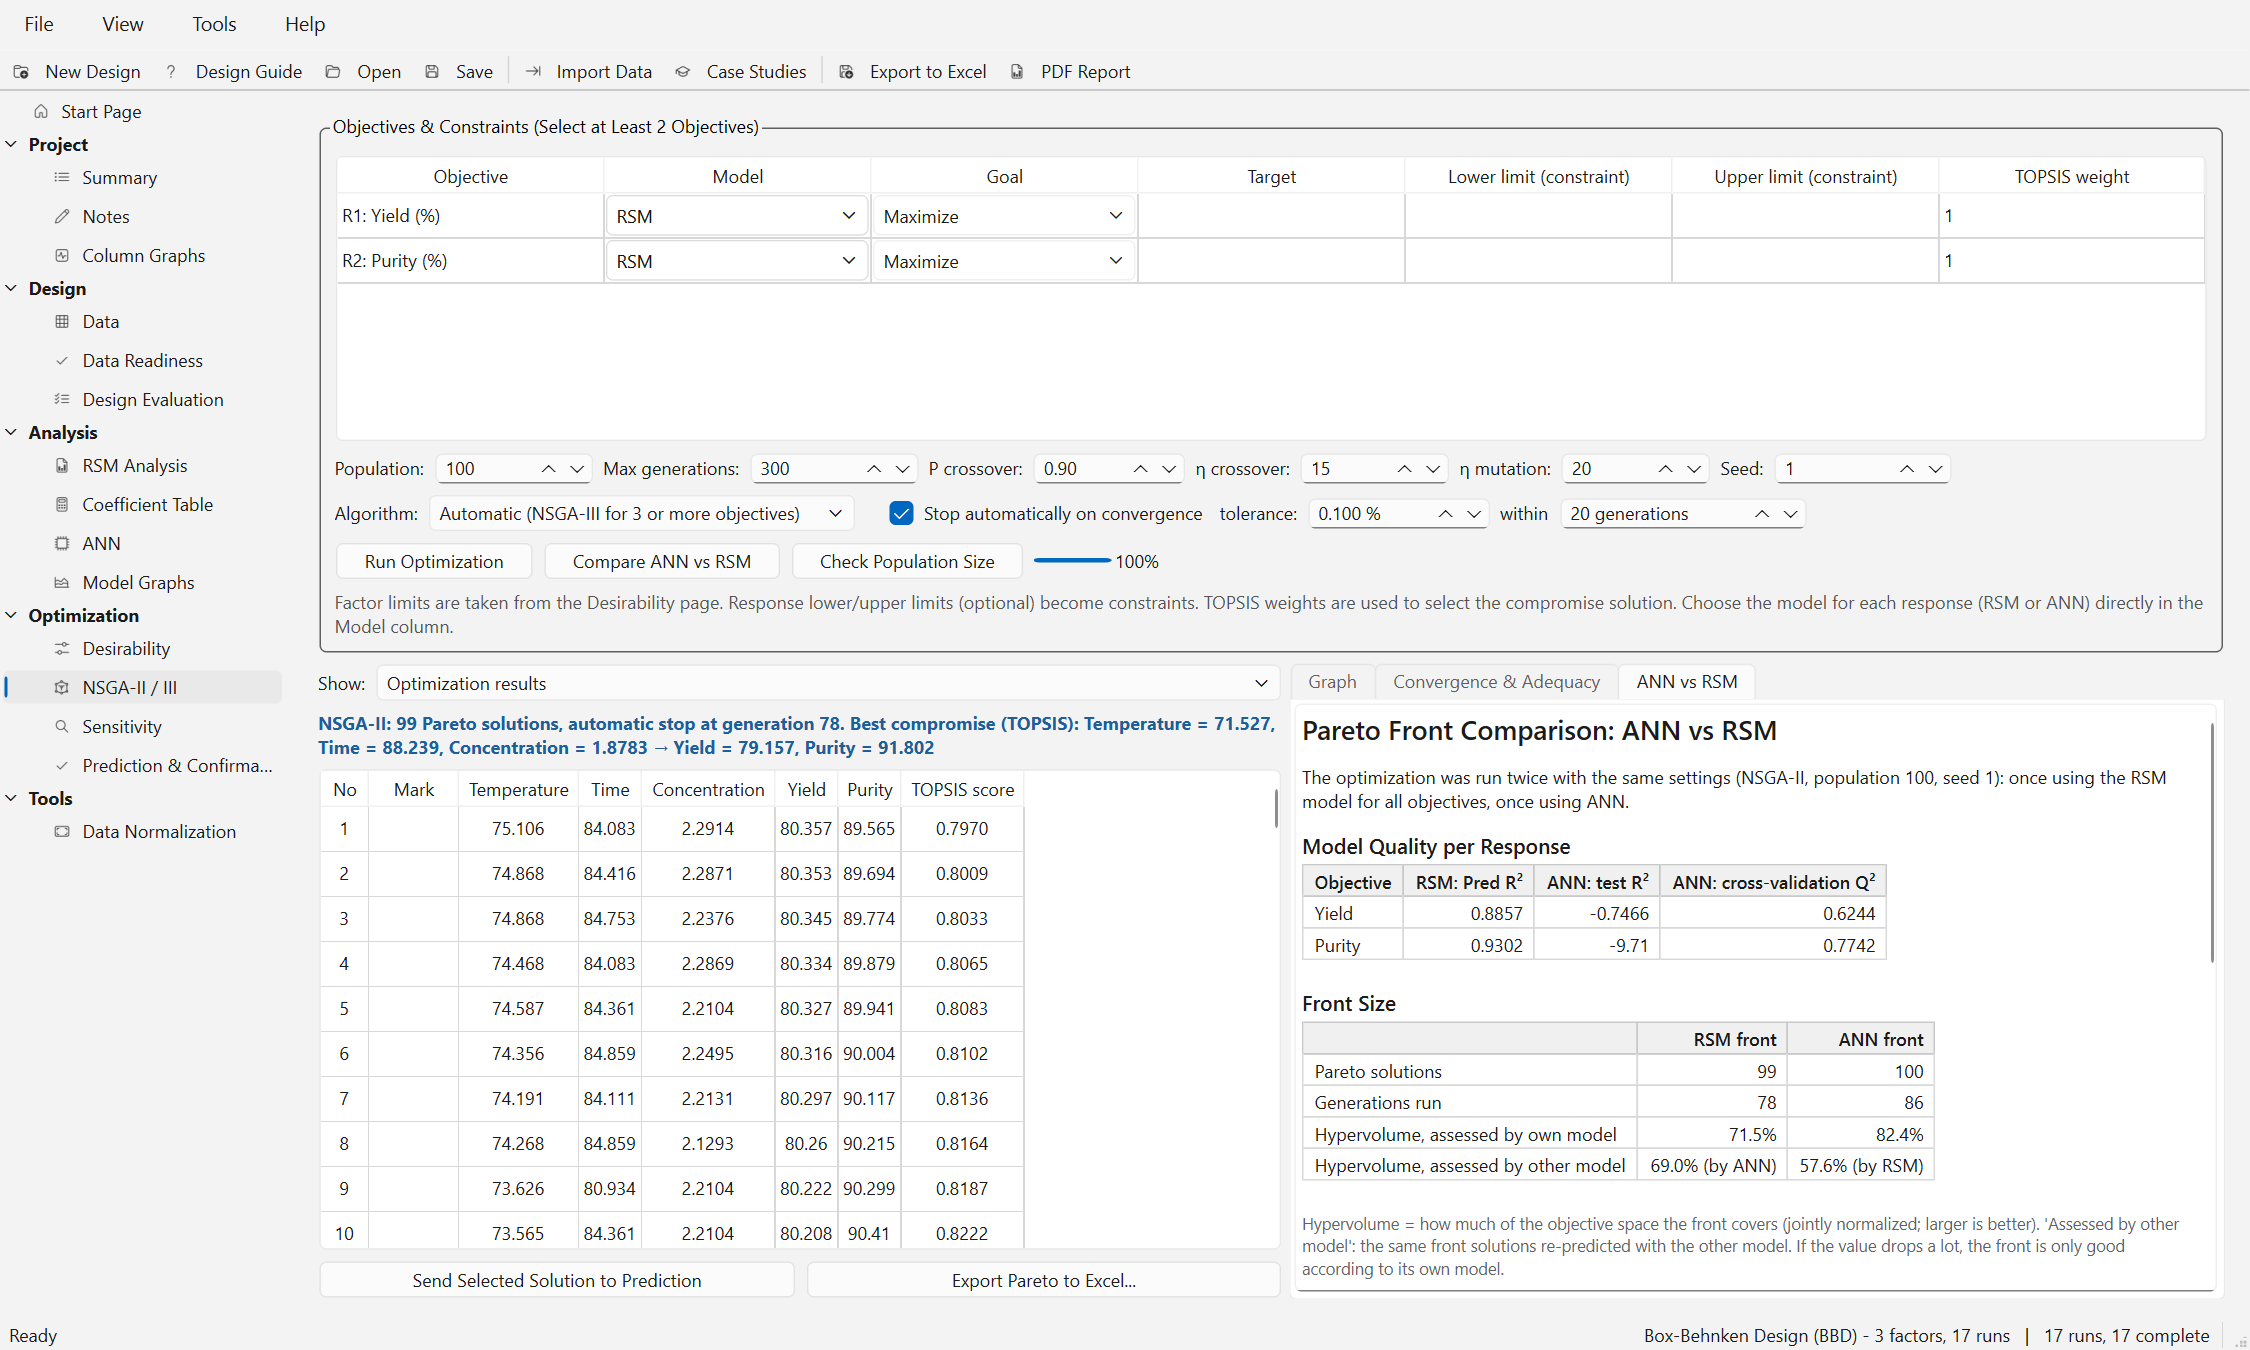
\includegraphics[width=\linewidth]{nsga_compare_report.png}
\caption{\ui{ANN vs RSM} report for the BBD case (upper part).}
\label{fig:ch08-cmp-report}
\end{figure}

The report gives:
\begin{itemize}
  \item Model quality: RSM predicted $R^2$ 0.8857 (Yield) and 0.9302 (Purity); ANN test $R^2$ $-0.7466$ and $-9.71$
        on the single final split (3 test runs each); ANN cross-validation $Q^2$ 0.6244 and 0.7742.
  \item Front size: 99 and 100 solutions, 78 and 86 generations. Hypervolume assessed by the own model 71.5~\% (RSM)
        and 82.4~\% (ANN); assessed by the other model 69.0~\% (RSM front by ANN) and 57.6~\% (ANN front by RSM).
  \item Prediction difference: Yield 22.4~\% mean, 78.0~\% maximum; Purity 4.3~\% mean, 9.9~\% maximum.
  \item TOPSIS choices: RSM front 71.527~°C, 88.239~min, 1.8783~\% (Yield 79.157 by RSM, 79.795 by ANN; Purity
        91.802 / 91.123); ANN front 65.325~°C, 89.999~min, 2.9973~\% (Yield 73.973 by RSM, 83.542 by ANN; Purity
        91.570 / 92.102). Distance $dx=56.0$~\%.
\end{itemize}
The conclusion is red: \ui{The models differ considerably: the largest mean difference of the predictions on the
front is 22.4\%, above the 10\% limit for partial agreement, and the compromise choices are 56\% of the factor range
apart, above the 15\% limit. Do not rely on just one model: make confirmation runs at both TOPSIS points.} It adds that
the ANN front promises the better trade-off by its own model but loses a lot of hypervolume when assessed by RSM,
and it compares the accuracy on new data: RSM mean Pred R² 0.908 against ANN mean cross-validation Q² 0.699 (both
ANNs were found by a search, so the cross-validated value is used).

\textbf{Interpretation.} Check~D fails here, and the reasons are clear. The ANN front reaches a Yield of about 84,
well above the highest observed Yield (78.29), at a corner of the design region (Time 90~min, Concentration 3~\%)
where the BBD has no run: this is extrapolation by a network trained on 17 runs. The RSM model has the better
accuracy on new data (predicted $R^2$ 0.886 and 0.930 against cross-validated $Q^2$ 0.624 and 0.774), and its front
loses little hypervolume when re-assessed by the ANN (71.5 to 69.0~\%). The RSM result is therefore the one to use,
and the disagreement is reported. If the ANN's promise matters, one or two confirmation runs at the ANN TOPSIS
setting decide the question; the RSM 95~\% prediction interval for the mean of three runs there is 72.1--75.8 for
Yield, far from the ANN prediction of 83.5 (see Chapter~\ref{chap:11}).

The single-split test $R^2$ values in the report ($-0.75$ and $-9.71$) are not a fair measure here: with 17 runs
the final split holds only three test runs, and one unusual run dominates $R^2$. Use the cross-validated $Q^2$.

\subsection{Limitations of check D}
Check~D compares two models; agreement does not prove that both are right, it only shows that the conclusion does not
depend on the model type. The prediction differences are measured on the Pareto solutions, which are often at the
edges of the design region where models are least reliable. For POE objectives the range $R_o$ is that of the
predictions, not of data. Finally, both NSGA runs use the same seed, so the comparison is reproducible but reflects one
realization of each front; check~C applies to each of them.
